\documentclass[aspectratio=169,11pt,hyperref={colorlinks=true}]{beamer}
\usetheme{boxes}
\setbeamertemplate{navigation symbols}{}
\definecolor{ibm}{RGB}{70,107,176}
\setbeamercolor{titlelike}{fg=ibm}
\setbeamercolor{structure}{fg=ibm}
\hypersetup{colorlinks,urlcolor=ibm}
\setbeamertemplate{footline}[frame number]
% Inserting graphics
\usepackage{graphicx}
% Side-by-side figures, etc
\usepackage{subfigure}
% Code snippits
\usepackage{listings}

\usepackage{lmodern}
% Color stuff
\usepackage{color}
\usepackage{amsmath}
\usepackage{amssymb}
\usepackage{empheq}
\usepackage[braket, qm]{qcircuit}
\usepackage{tikz}
\usepackage{gensymb}
\newcommand\RBox[1]{%
  \tikz\node[draw,rounded corners,align=center,] {#1};%
}
\usepackage{hyperref}
%\usecolortheme{buzz}
%\usecolortheme{wolverine}
%\usetheme{Boadilla}
\usepackage[T1]{fontenc}

\definecolor{mygreen}{rgb}{0,0.6,0}
\definecolor{mygray}{rgb}{0.5,0.5,0.5}
\definecolor{mymauve}{rgb}{0.58,0,0.82}

\lstset{%
  backgroundcolor=\color{white},   % choose the background color; you must add \usepackage{color} or \usepackage{xcolor}
  breakatwhitespace=false,         % sets if automatic breaks should only happen at whitespace
  breaklines=true,                 % sets automatic line breaking
  captionpos=b,                    % sets the caption-position to bottom
  commentstyle=\color{ibm},  % comment style
  extendedchars=true,              % lets you use non-ASCII characters; for 8-bits encodings only, does not work with UTF-8
  keepspaces=true,                 % keeps spaces in text, useful for keeping indentation of code (possibly needs columns=flexible)
  keywordstyle=\color{blue},       % keyword style
%  otherkeywords={*,...},           % if you want to add more keywords to the set
  numbersep=5pt,                   % how far the line-numbers are from the code
  numberstyle=\tiny\color{mygray}, % the style that is used for the line-numbers
  rulecolor=\color{black},         % if not set, the frame-color may be changed on line-breaks within not-black text (e.g. comments (green here))
  showspaces=false,                % show spaces everywhere adding particular underscores; it overrides 'showstringspaces'
  showstringspaces=false,          % underline spaces within strings only
  showtabs=false,                  % show tabs within strings adding particular underscores
  stringstyle=\color{ibm},   % string literal style
}


\setbeamerfont{caption}{series=\normalfont,size=\fontsize{6}{8}}
\setbeamertemplate{caption}{\raggedright\insertcaption\par}

\setlength{\abovecaptionskip}{0pt}
\setlength{\floatsep}{0pt}

\author[Matthew Treinish]{%
    \texorpdfstring{%
        \centering
        Matthew Treinish\\
        Software Engineer - IBM Research\\
        \href{mailto:mtreinish@kortar.org}{mtreinish@kortar.org}\\
        \texttt{mtreinish on Freenode}\\
        \href{https://github.com/mtreinish/open-source-quantum-computing/tree/fossc-2019}{https://github.com/mtreinish/open-source-quantum-computing/tree/fossc-2019}
   }
   {Matthew Treinish}
}
\date{}

\title{Open Source Quantum Computing}
\begin{document}

{
\setbeamertemplate{background canvas}{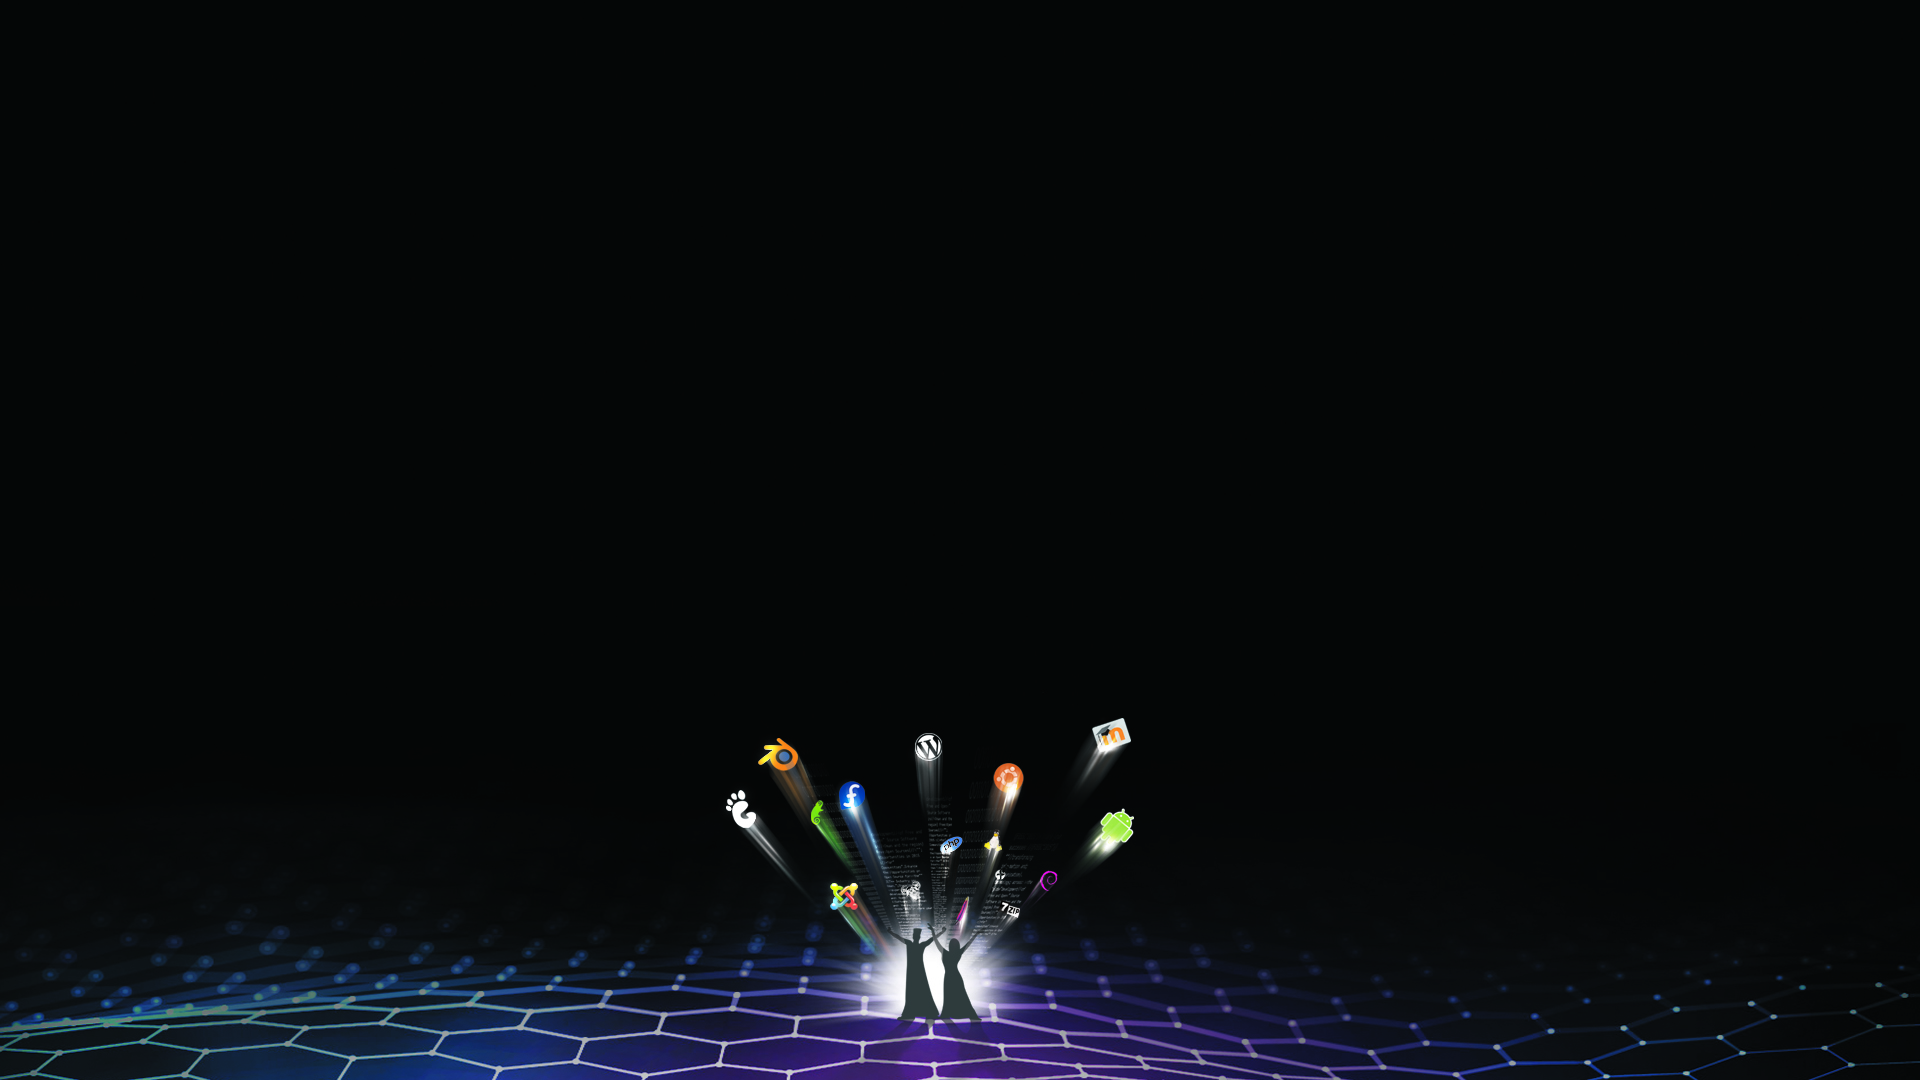
\includegraphics[width=\paperwidth,height=\paperheight]{fossc-title.png}}
\setbeamertemplate{footline}{}
\begin{frame}[noframenumbering]
    \setbeamercolor{titlelike}{fg=white}
    \setbeamercolor{structure}{fg=white}
    \setbeamercolor{normal text}{fg=white}
    \hypersetup{colorlinks,urlcolor=white}
    \setbeamercolor{author}{fg=white}
    \setbeamercolor{date}{fg=white}
    \setbeamercolor{background}{bg=black}
    \titlepage{}
\end{frame}
}

%\usebackgroundtemplate{
%    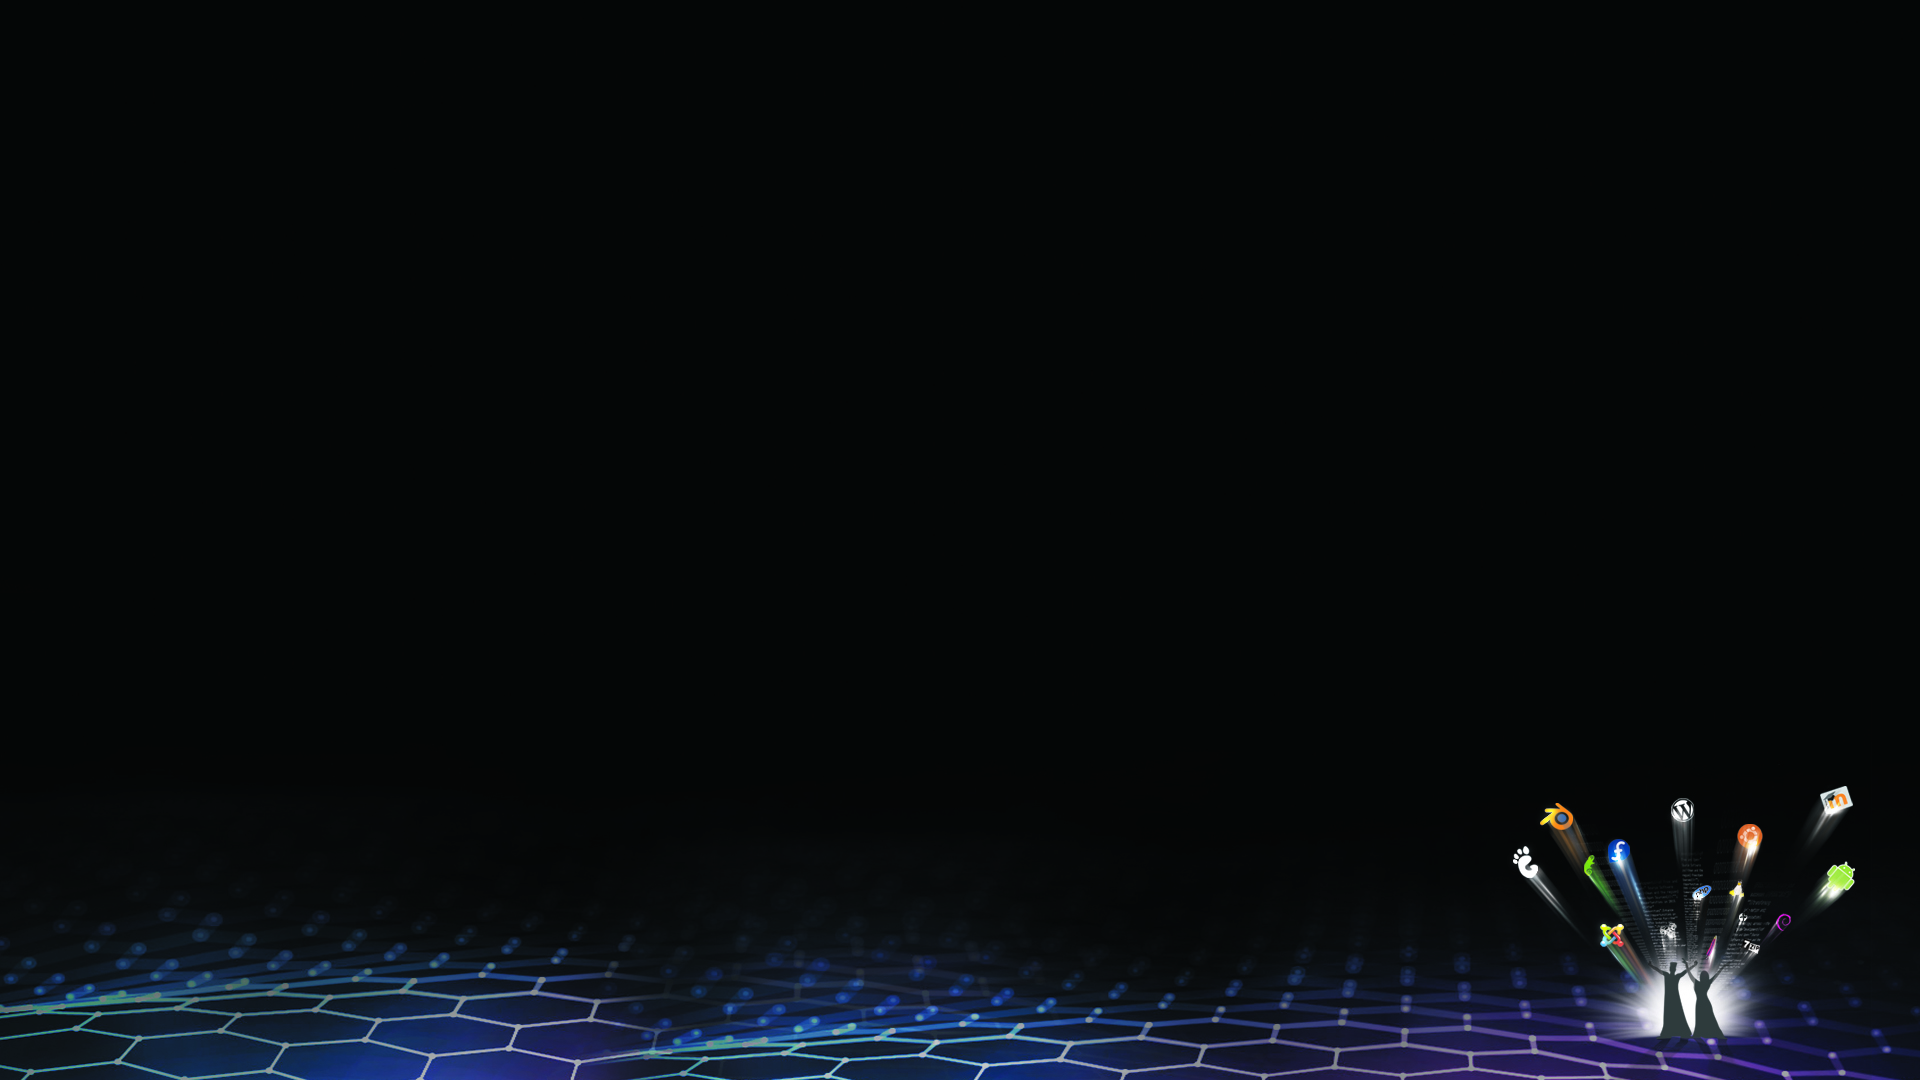
\includegraphics[width=\paperwidth,height=\paperheight]{fossc-background.png}}
\section{What is a Quantum Computer}
\newcommand{\iu}{{i\mkern1mu}}

\begin{frame}
    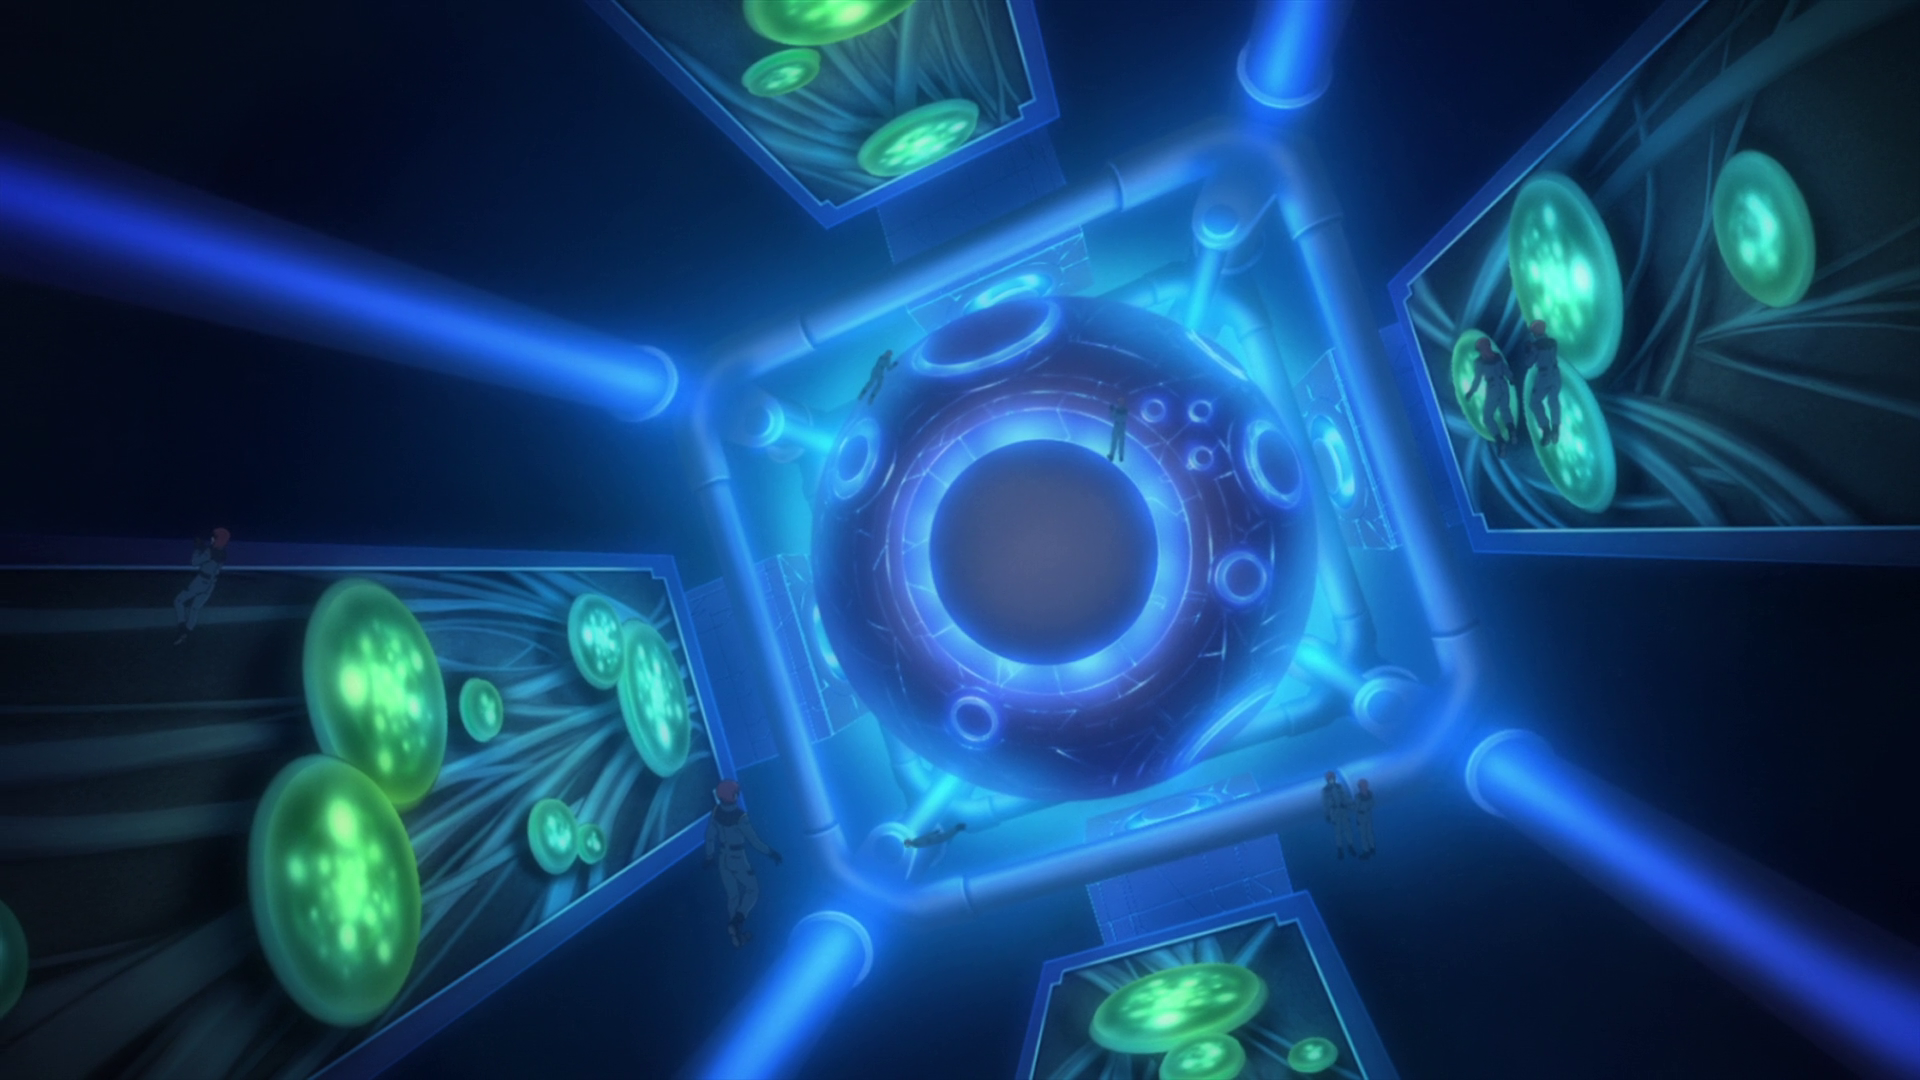
\includegraphics[width=\textwidth]{Veda_AD2314.png}
\end{frame}

\begin{frame}
    \frametitle{Real Quantum Computer}
    \begin{columns}[t]
        \column{.5\textwidth}
            \centering
            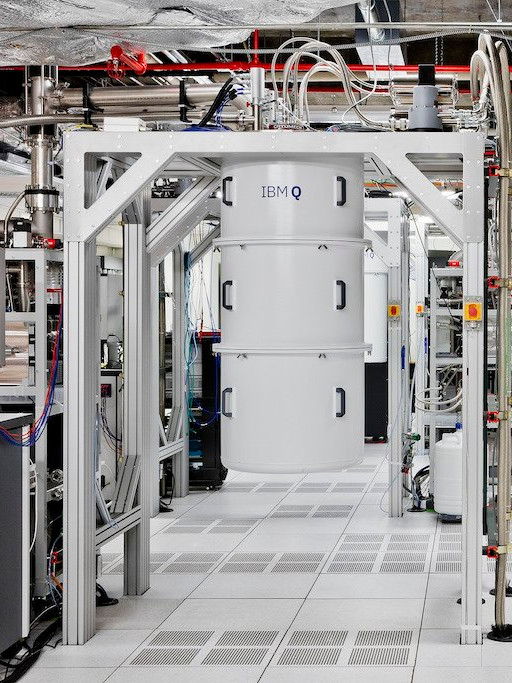
\includegraphics[height=.45\textheight]{outside.jpg}\\
            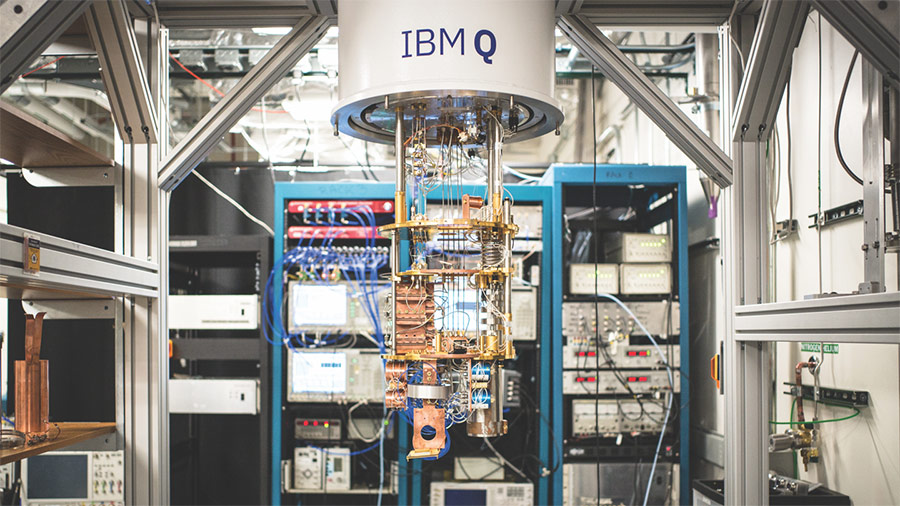
\includegraphics[height=.45\textheight]{inside-1.jpg}
        \column{.5\textwidth}
            \centering
            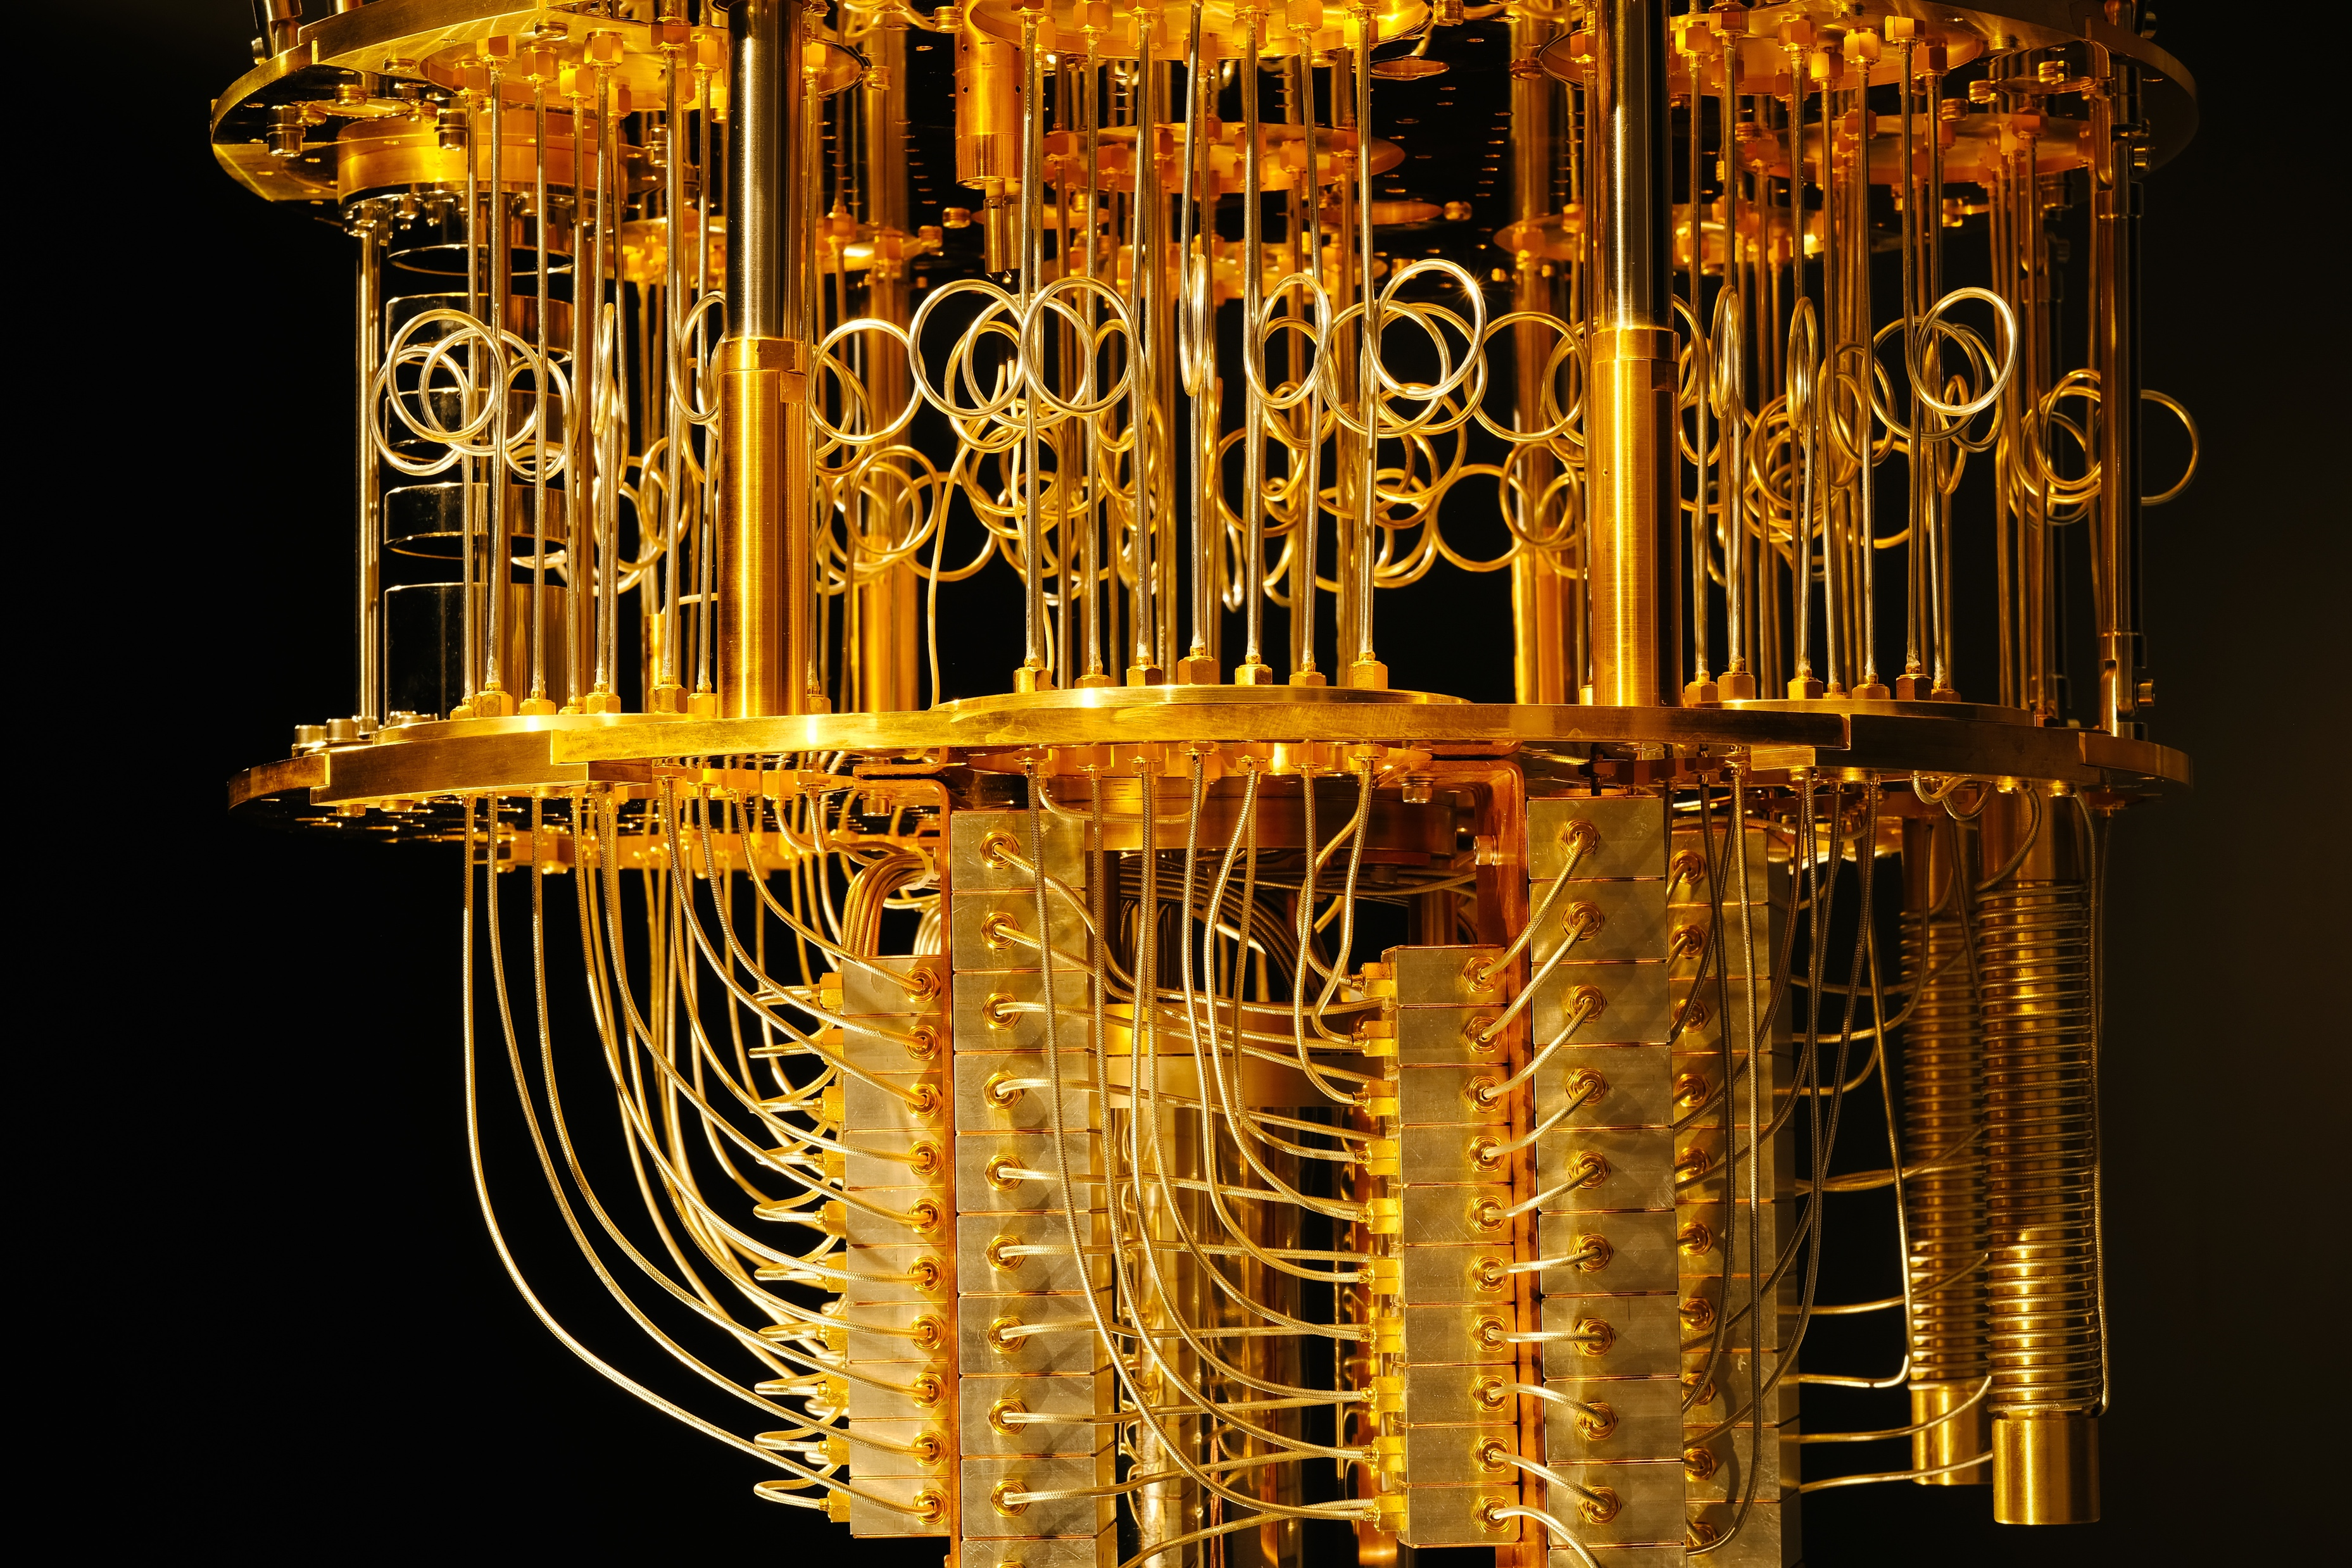
\includegraphics[height=.45\textheight]{fridge.jpg}\\
            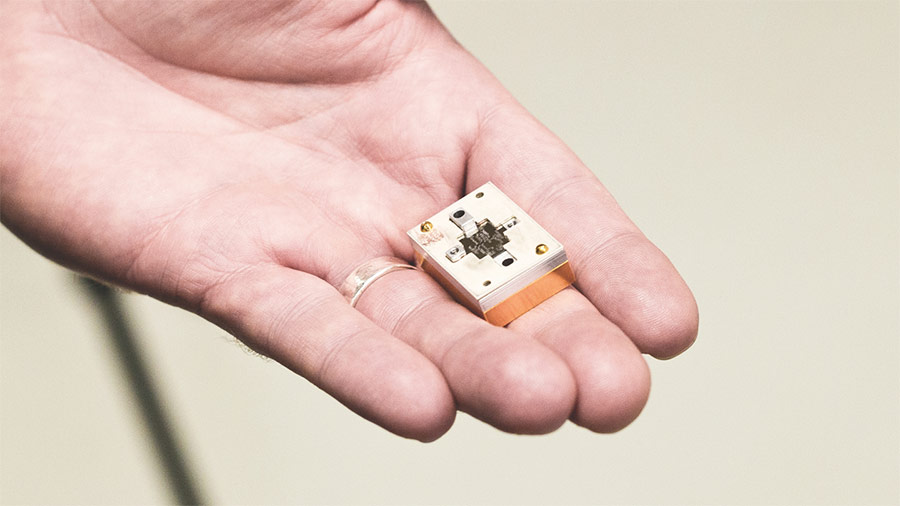
\includegraphics[height=.45\textheight]{inside-4.jpg}
    \end{columns}
\end{frame}

\begin{frame}
    \frametitle{Quantum Chips}
    \begin{columns}
        \column{.45\linewidth}
            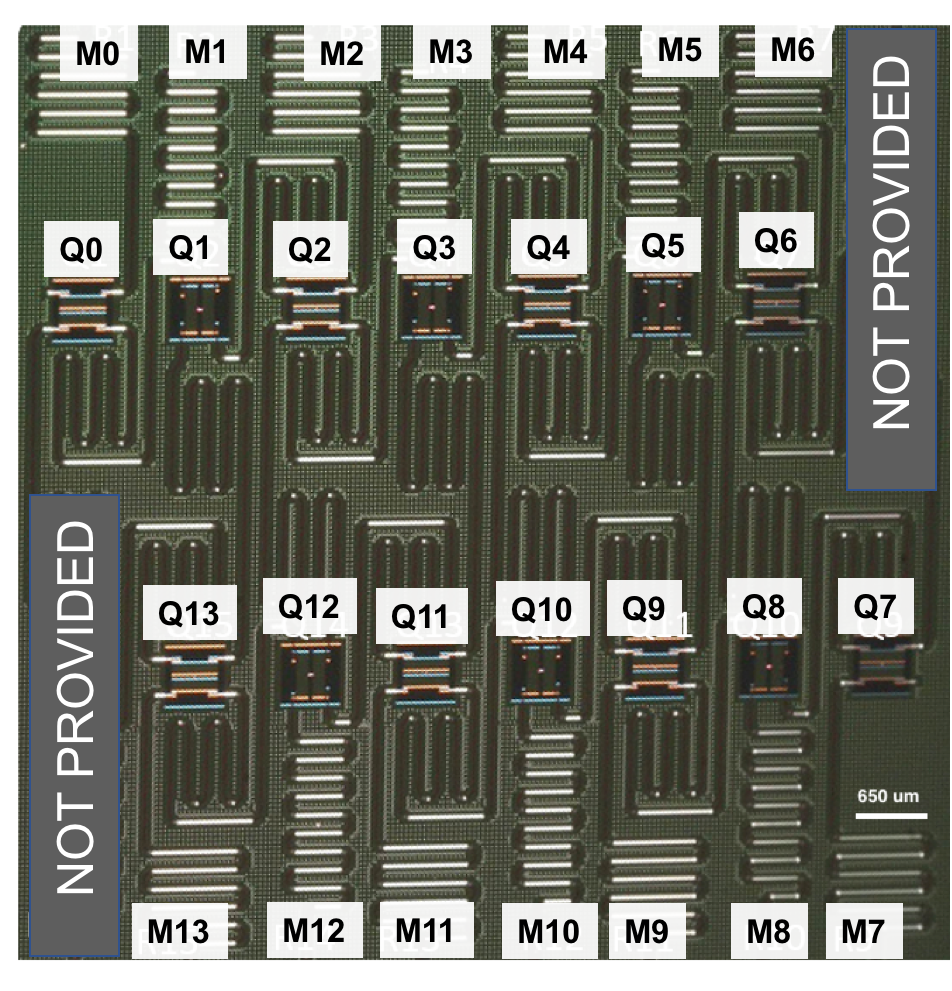
\includegraphics[width=\textwidth]{melbourne-labeled.png}
        \column{.45\linewidth}
            \includegraphics[width=\textwidth]{ibmqx4-labeled.png}
    \end{columns}
    \centering
    \href{https://github.com/Qiskit/ibmq-device-information}{https://github.com/Qiskit/ibmq-device-information}
\end{frame}

\begin{frame}
    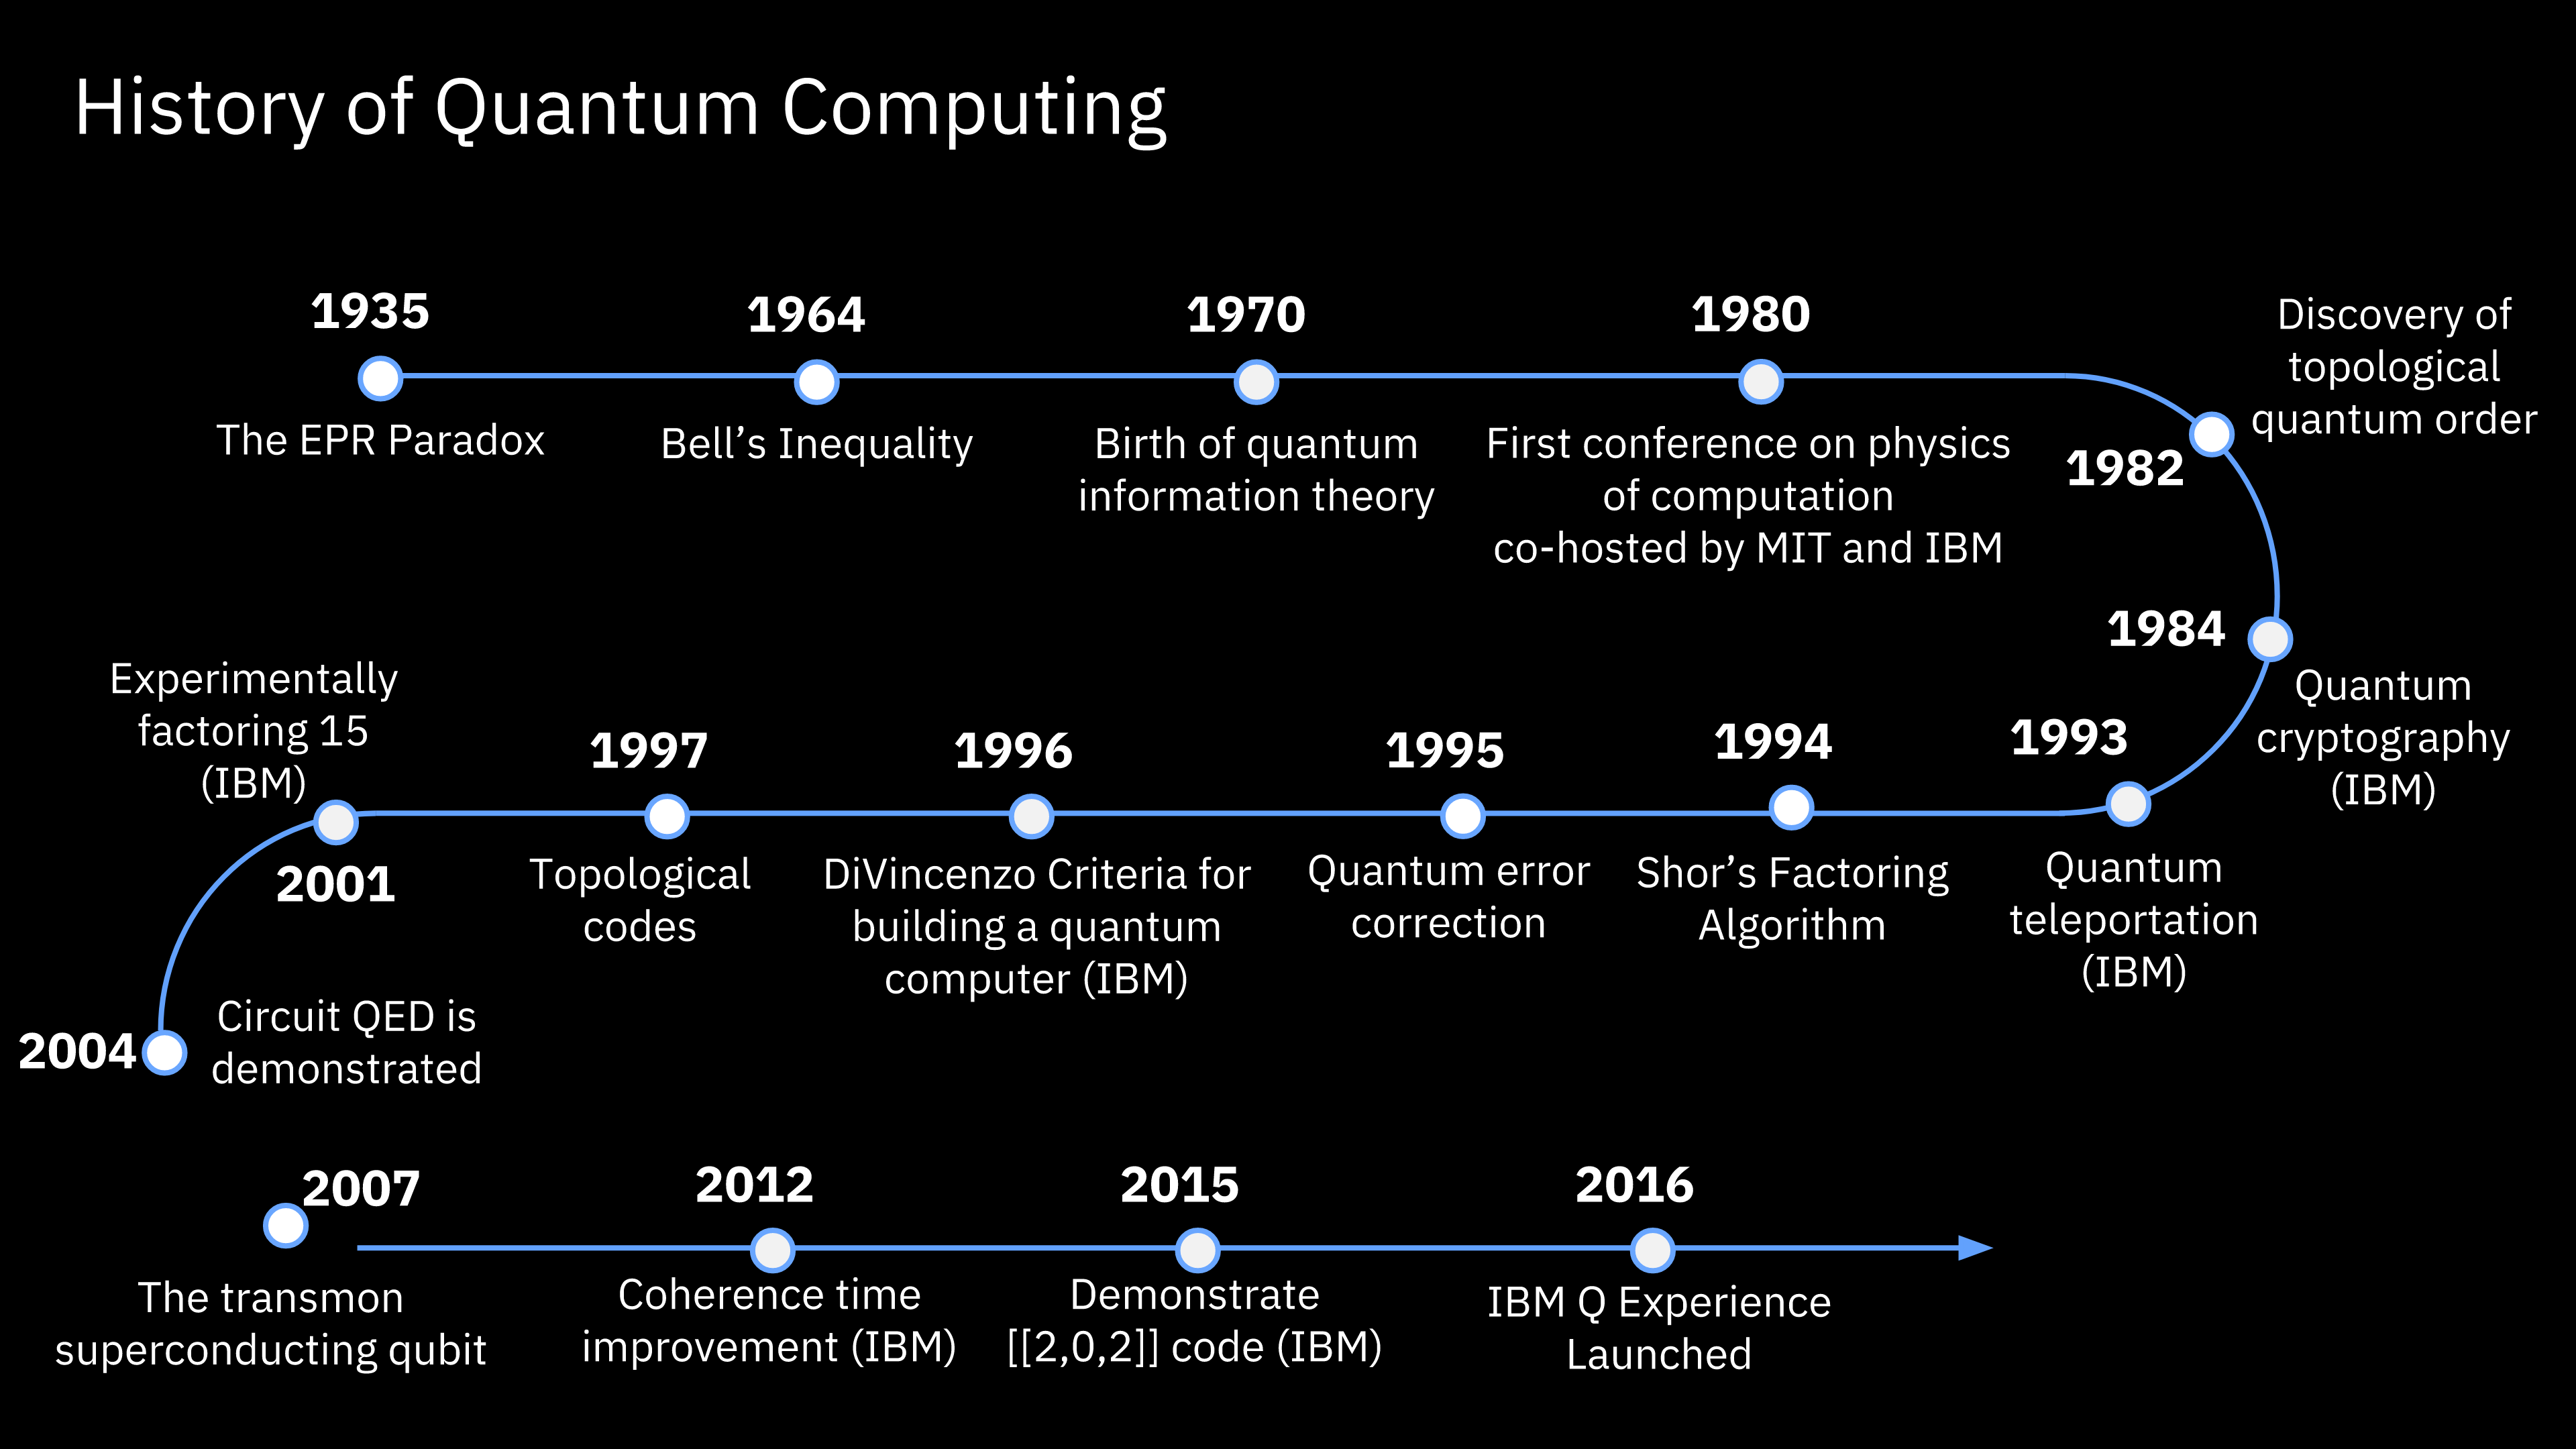
\includegraphics[width=\textwidth]{timeline.png}
\end{frame}

\begin{frame}
    \frametitle{What is Qiskit?}
    \begin{columns}
        \column{.5\textwidth}
            \begin{itemize}
                \item SDK for working with Noisy Intermediate-Scale Quantum (NISQ) computers
                \item Apache 2.0 License
                \item Designed to be backend agnostic
                \item Includes out-of-the-box local simulators and support for running on IBMQ
            \end{itemize}
        \column{.5\textwidth}
            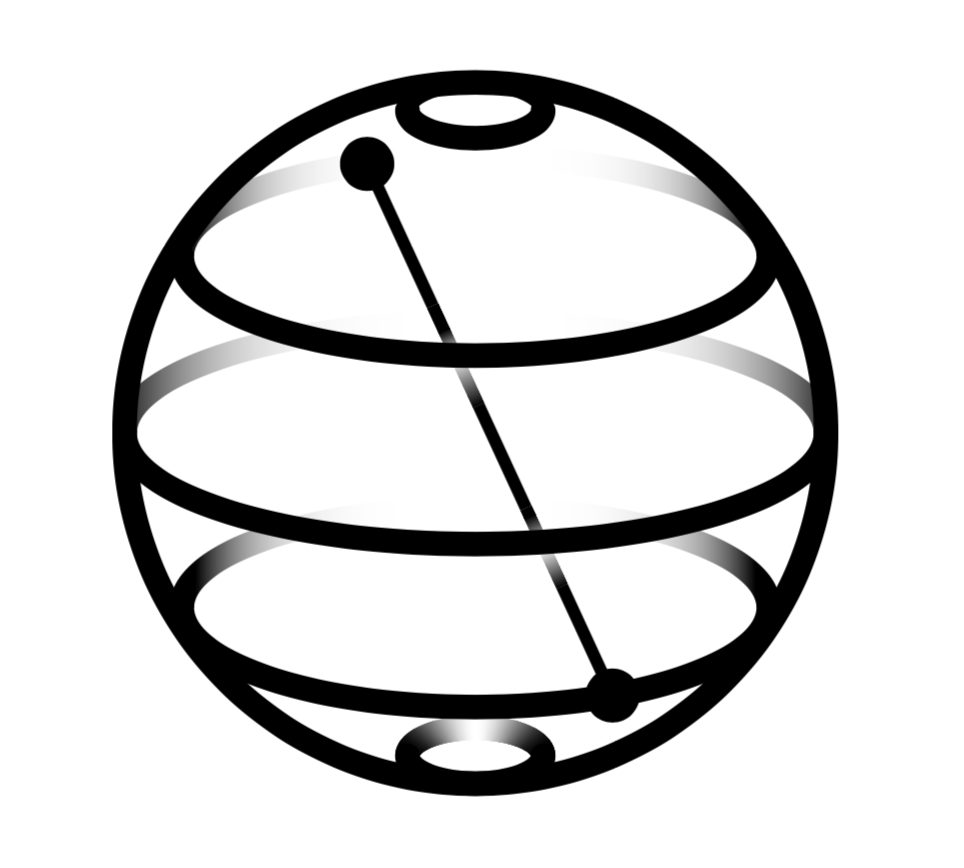
\includegraphics[width=\textwidth]{qiskit_logo.png}
    \end{columns}
\end{frame}

\begin{frame}
    \frametitle{Qiskit Elements}
    \centering
    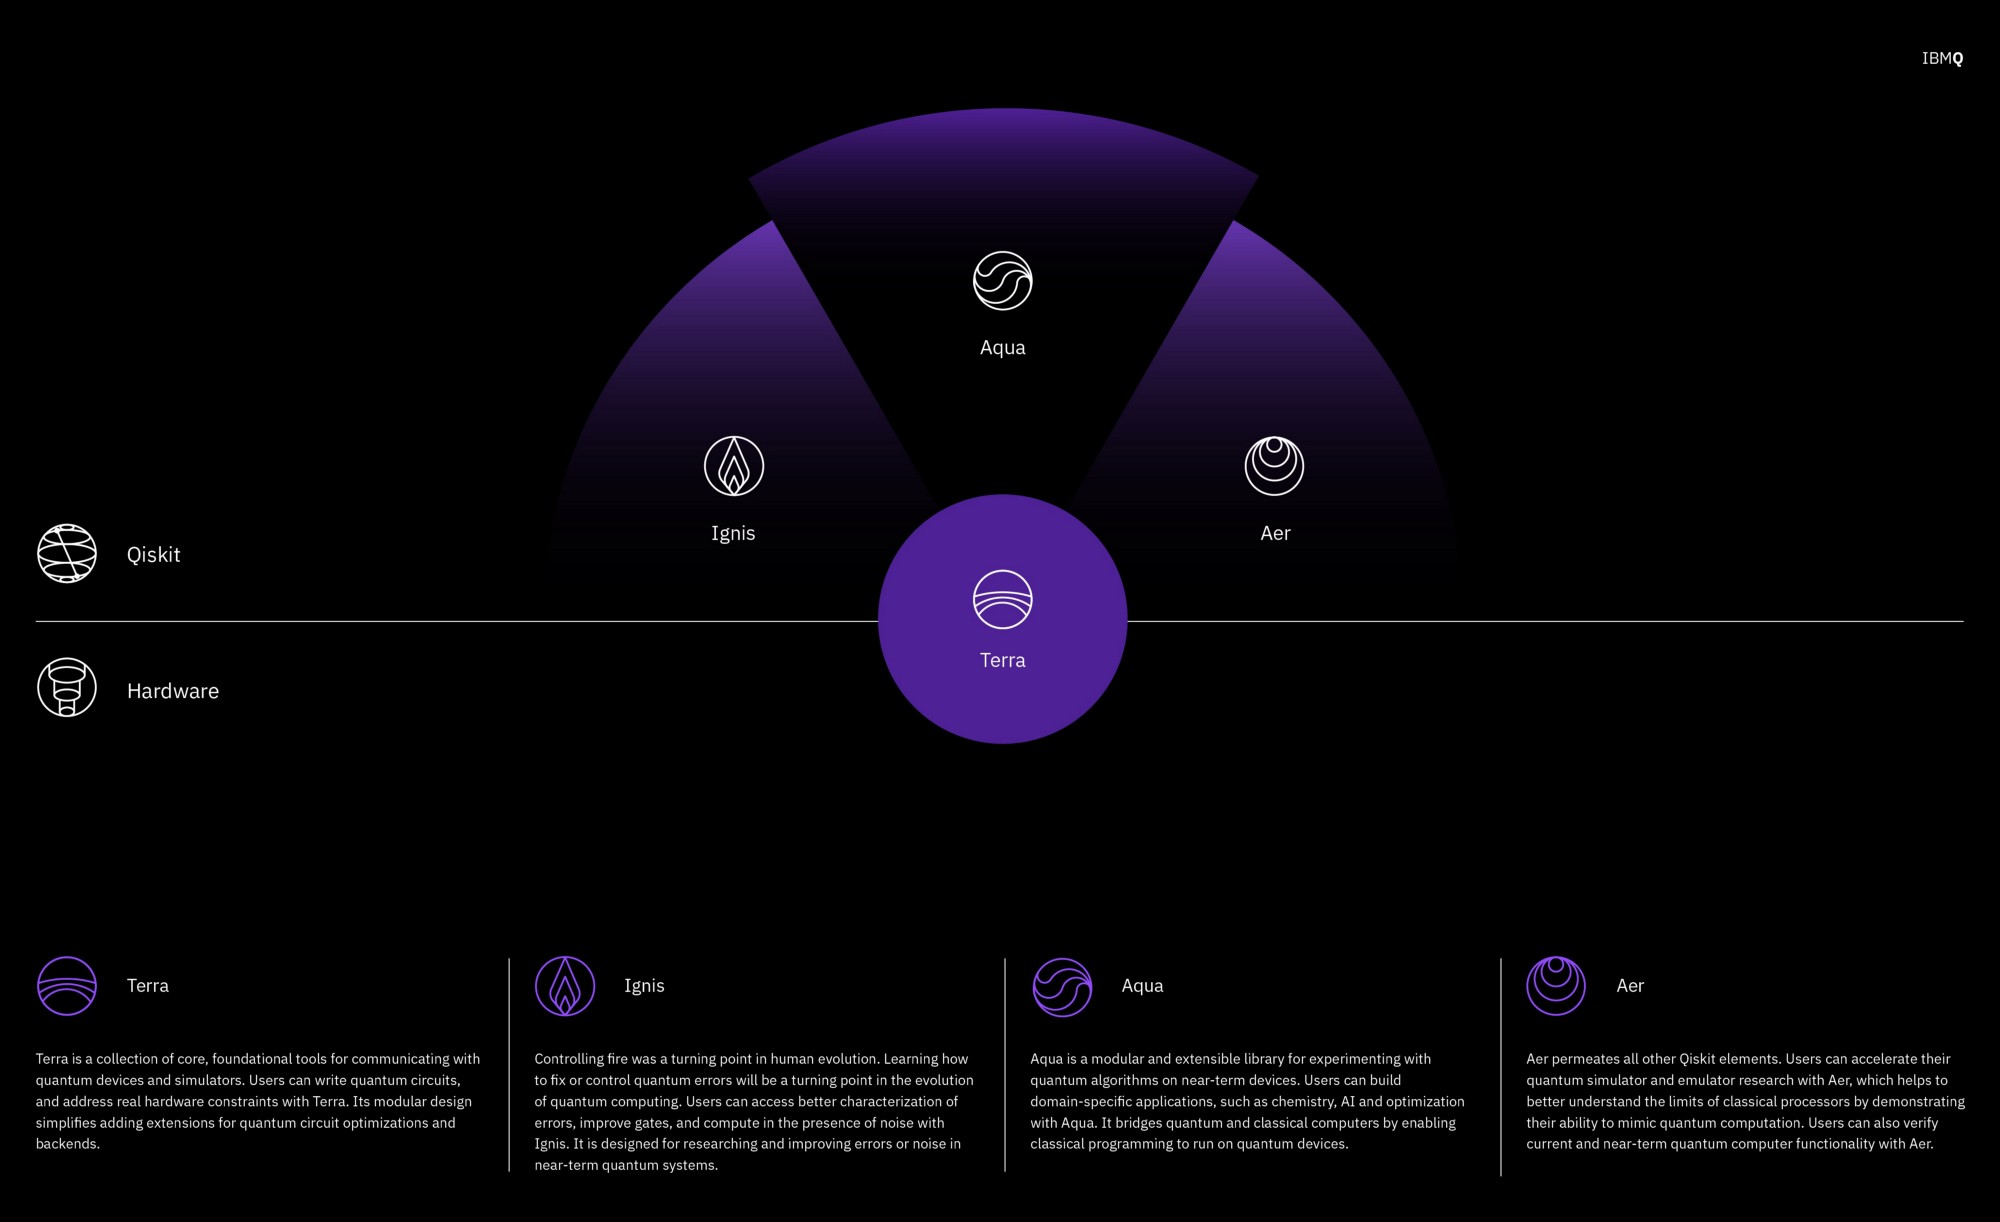
\includegraphics[width=.99\textwidth]{qiskit-components.jpeg}
\end{frame}

\begin{frame}
    \frametitle{Qiskit Terra}
    \begin{columns}
        \column{.5\textwidth}
           \begin{itemize}
                \item Is the base layer for applications, provides interface to hardware and simulators
                \item Provides an SDK for working with quantum circuits
                \item Compiles circuits to run on different backends
                \item Written in Python
           \end{itemize}
        \column{.5\textwidth}
            \centering
            \colorbox{black}{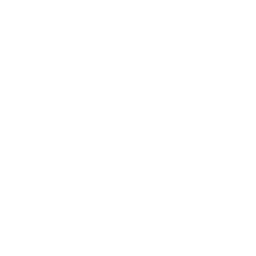
\includegraphics[width=.5\textwidth]{qiskit-terra-logo.png}}
    \end{columns}
\end{frame}

\section{Quantum Information Theory}
\subsection{The Qubit}
\begin{frame}
    \frametitle{The Qubit}
    \begin{columns}
        \column{.4\textwidth}
            \begin{itemize}
                \item The bloch sphere provides a representation of qubit state
                \item State can be at any point along surface of sphere
                \item Measuring a qubit occurs along the Z axis. (also called basis states)
                \item Measuring a qubit is irreversible and will either be 0
                      or 1
            \end{itemize}
        \column{.6\textwidth}
            \begin{center}
                \textbf{Bloch Sphere:}
                \only<1>{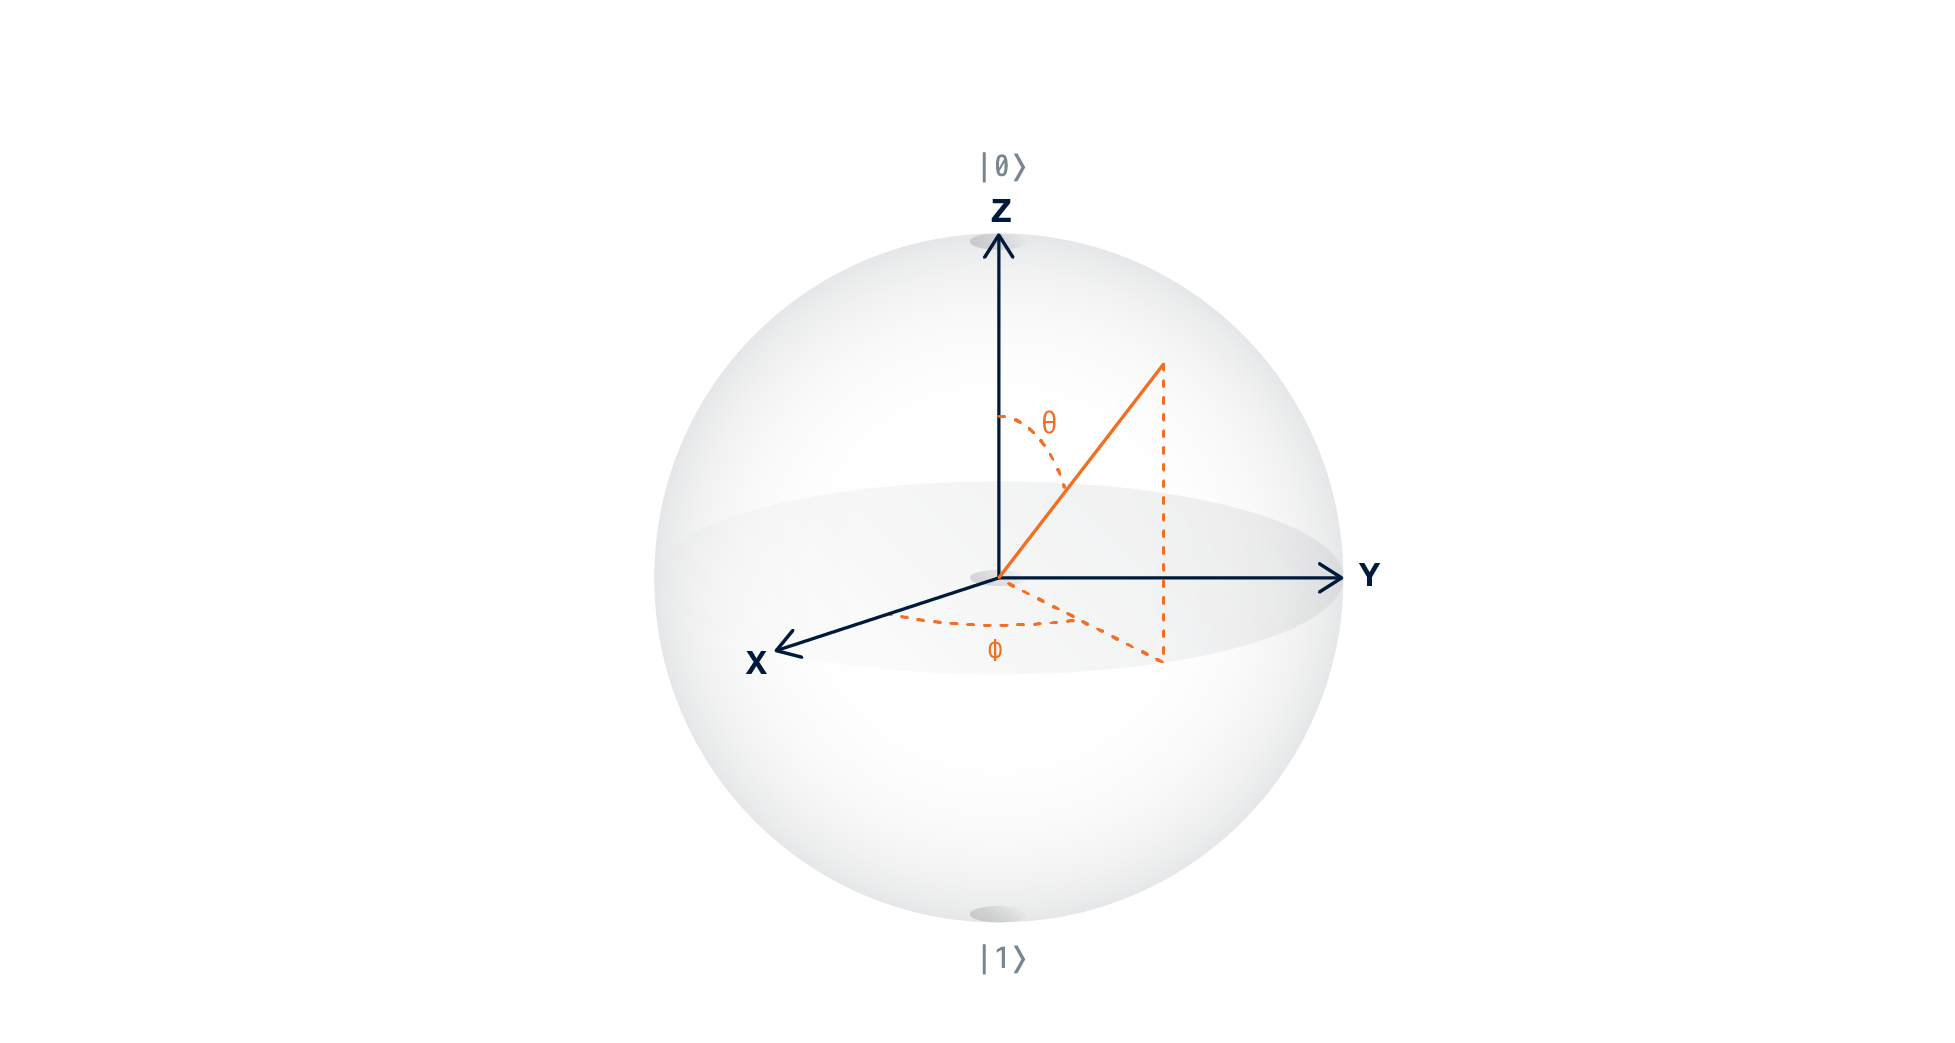
\includegraphics[height=.85\textheight]{bloch_angles.png}}
                \only<2>{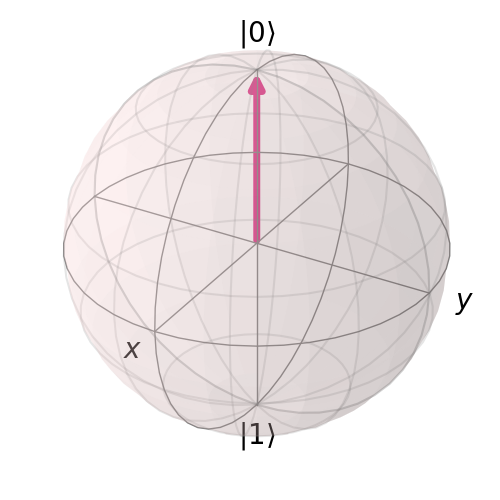
\includegraphics[height=.85\textheight]{bloch_fresh.png}}
                \only<3>{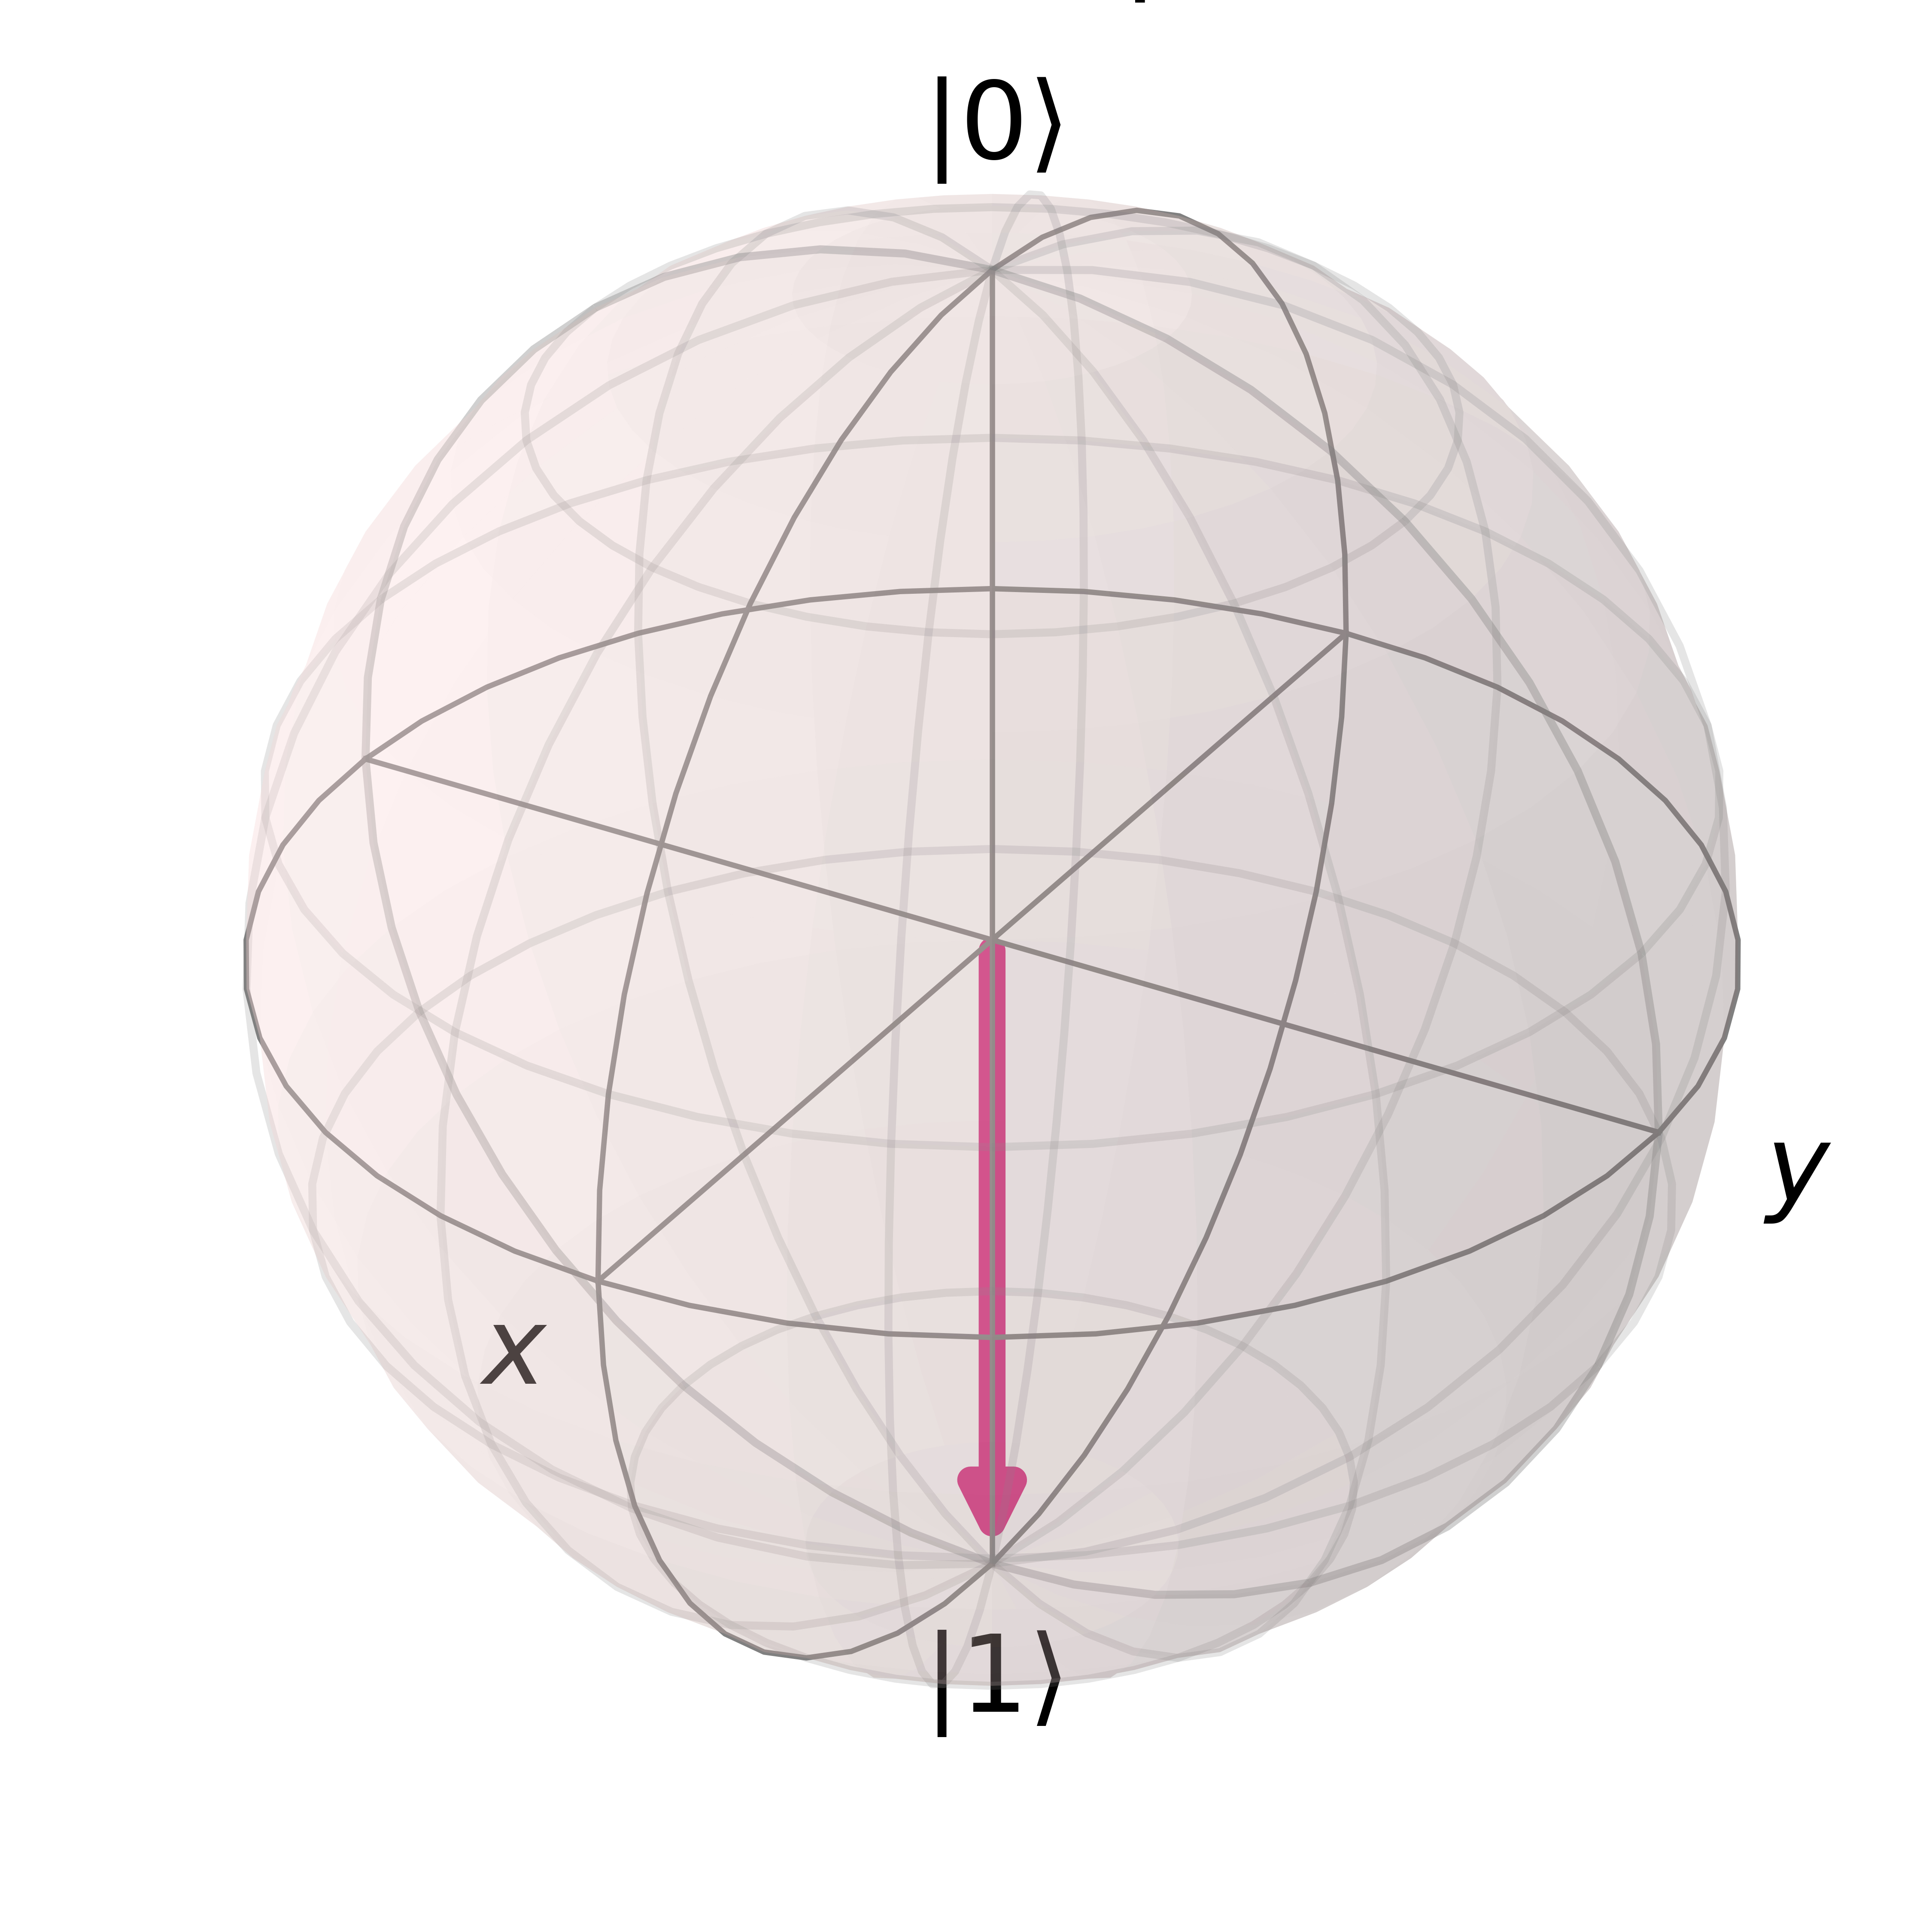
\includegraphics[height=.85\textheight]{bloch_one.png}}
        \end{center}
    \end{columns}
\end{frame}

\subsection{Quantum Gates}
\begin{frame}
    \frametitle{Quantum Gates}
    \begin{itemize}  
        \item Quantum Logic Gates are used perform operations on qubits
        \item Gates are reversible
        \item Gates can be represented as unitary matrices
    \end{itemize}
    \centering
    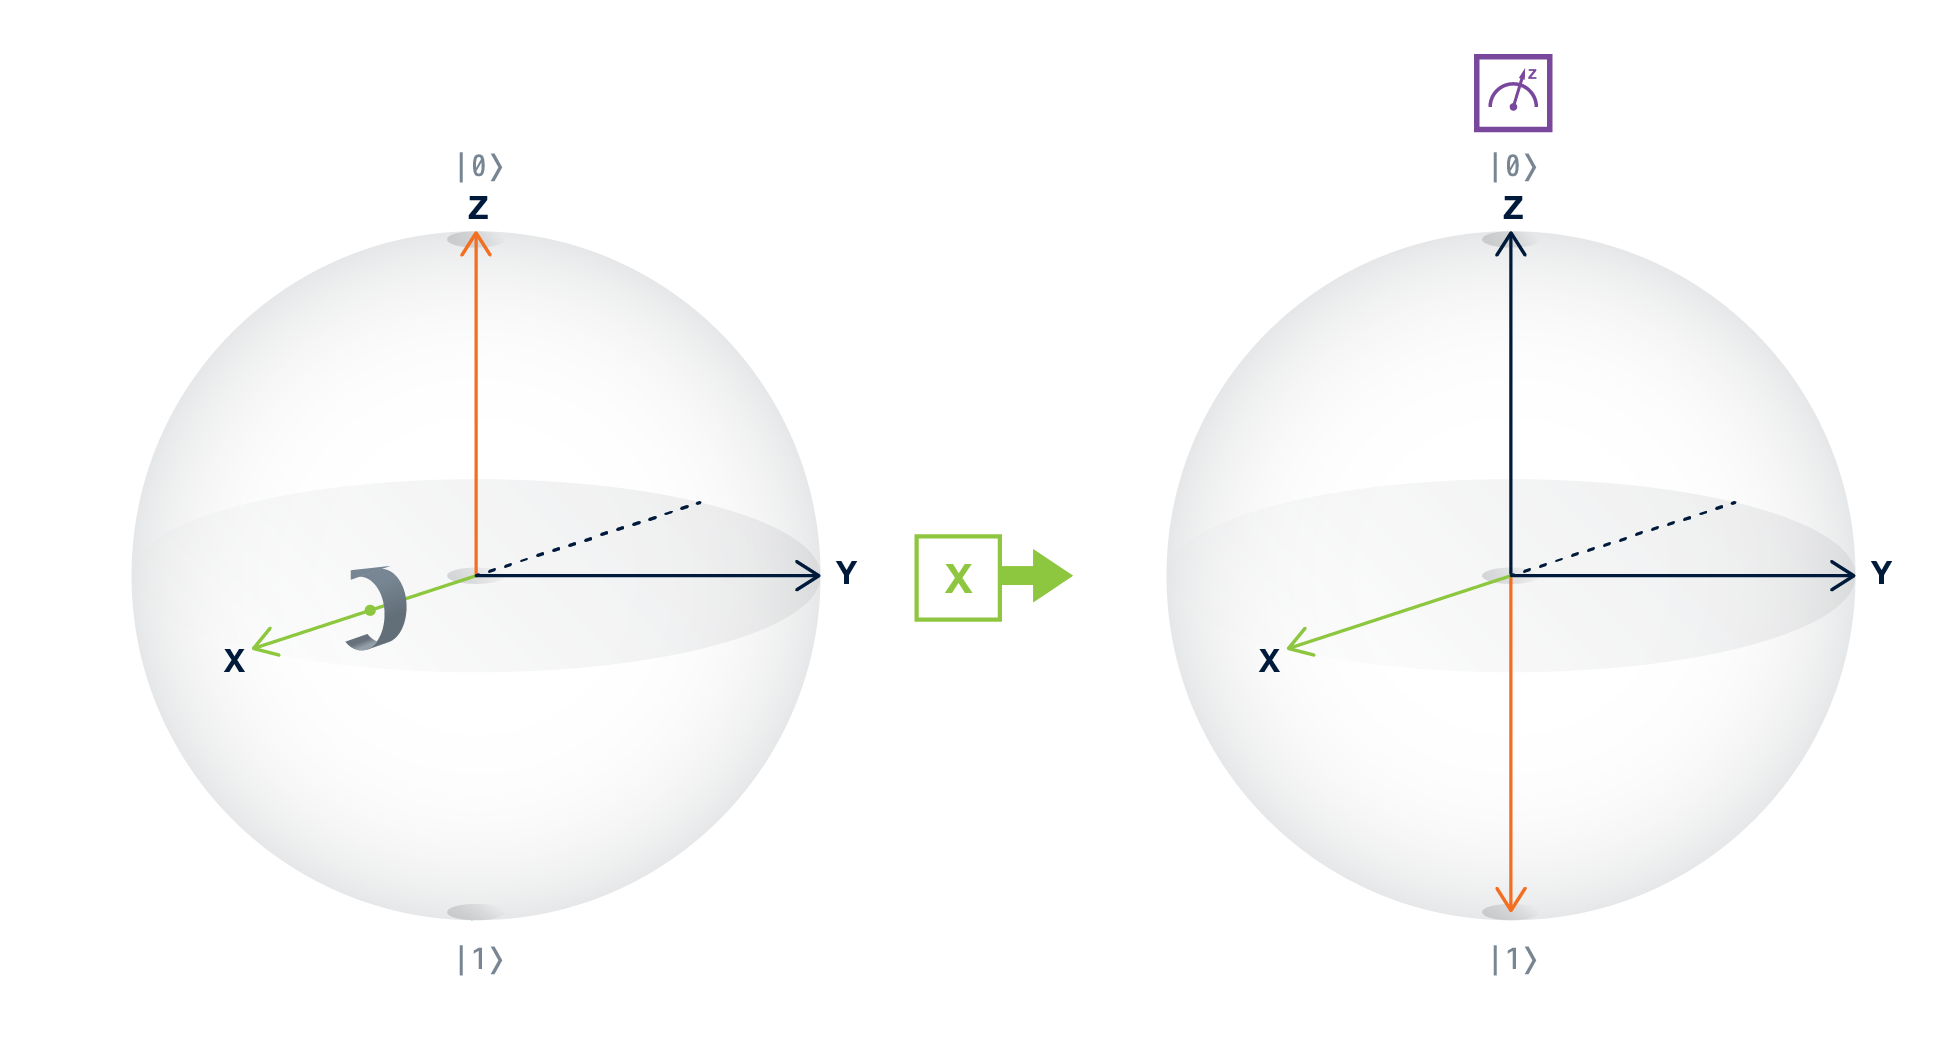
\includegraphics[width=.9\textwidth]{gate_x_bloch.png}
%    \begin{columns}[onlytextwidth]
%        \begin{column}{.333\textwidth}
%            \centering
%            \textbf{Gate}
%            \begin{equation*}
%                \Qcircuit @C=0.5em @R=0.0em @!R {
%	 	            \lstick{\ket{0}} & \gate{X} & \qw & \qw\\
%            	}
%            \end{equation*} \\
%        \end{column}
%        \begin{column}{.333\textwidth}
%            \centering
%            \textbf{Matrix Form}
%            \[\begin{bmatrix}
%                0 & 1\\
%                1 & 0 \\
%            \end{bmatrix}\]\\
%        \end{column}
%    \end{columns}
\end{frame}

\subsection{Superposition and Hadamards}
\begin{frame}
    \frametitle{Superposition}
    \begin{itemize}
    \item Identically prepared qubits can still behave randomly
    \item The randomness is inherent in nature
    \end{itemize}
    \begin{columns}
        \column{.5\textwidth}
            \centering
            \LARGE \textbf{$\ket{0}$} \\
            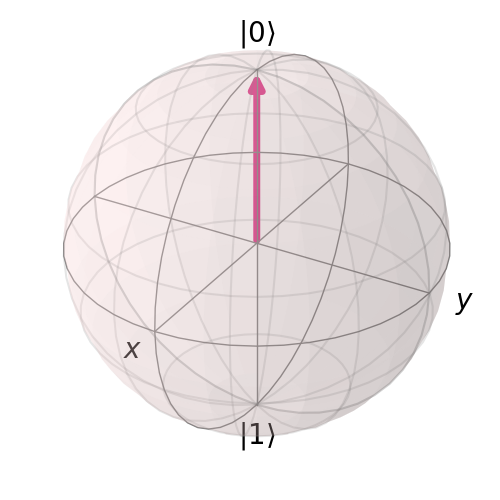
\includegraphics[width=.4\textwidth]{bloch_fresh.png} \\
            \LARGE \textbf{$\ket{1}$} \\
            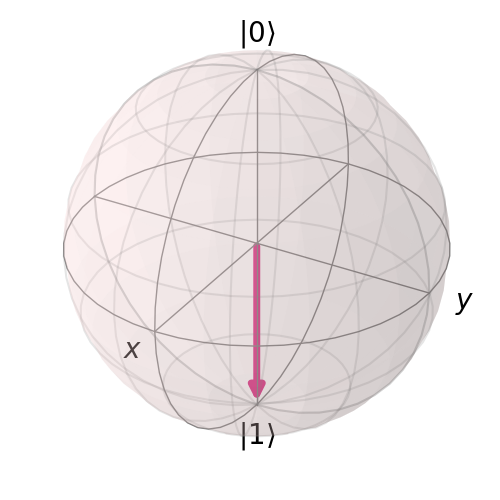
\includegraphics[width=.4\textwidth]{bloch_x.png}\\
        \column{.5\textwidth}
            \centering
            \LARGE \textbf{$\ket{0} + \ket{1}$} \\
            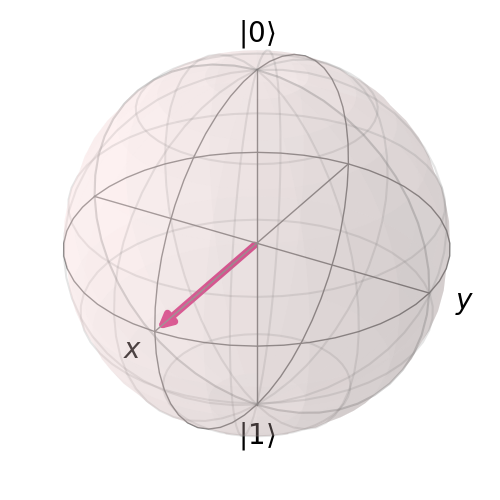
\includegraphics[width=.5\textwidth]{bloch_hadamard.png}\\
            \textbf{$\sim$50/50 chance of being \ket{0} or \ket{1}}
    \end{columns}
\end{frame}

\begin{frame}
    \frametitle{Hadamard Gate}
%    \begin{columns}
%        \column{.5\textwidth}
%        \centering
%        \textbf{Gate}
%        \begin{equation*}
%            \Qcircuit @C=0.5em @R=0.0em @!R {
%	 	        \lstick{\ket{0}} & \gate{H} & \qw & \qw\\
%    	     }
%        \end{equation*}
%        \column{.5\textwidth}
%        \centering
%        \textbf{Matrix Form}
%        \[\frac{1}{\sqrt{2}} \begin{bmatrix}
%            1 & 1 \\
%            1 & -1 \\
%        \end{bmatrix}\]
%    \end{columns}
    \centering
    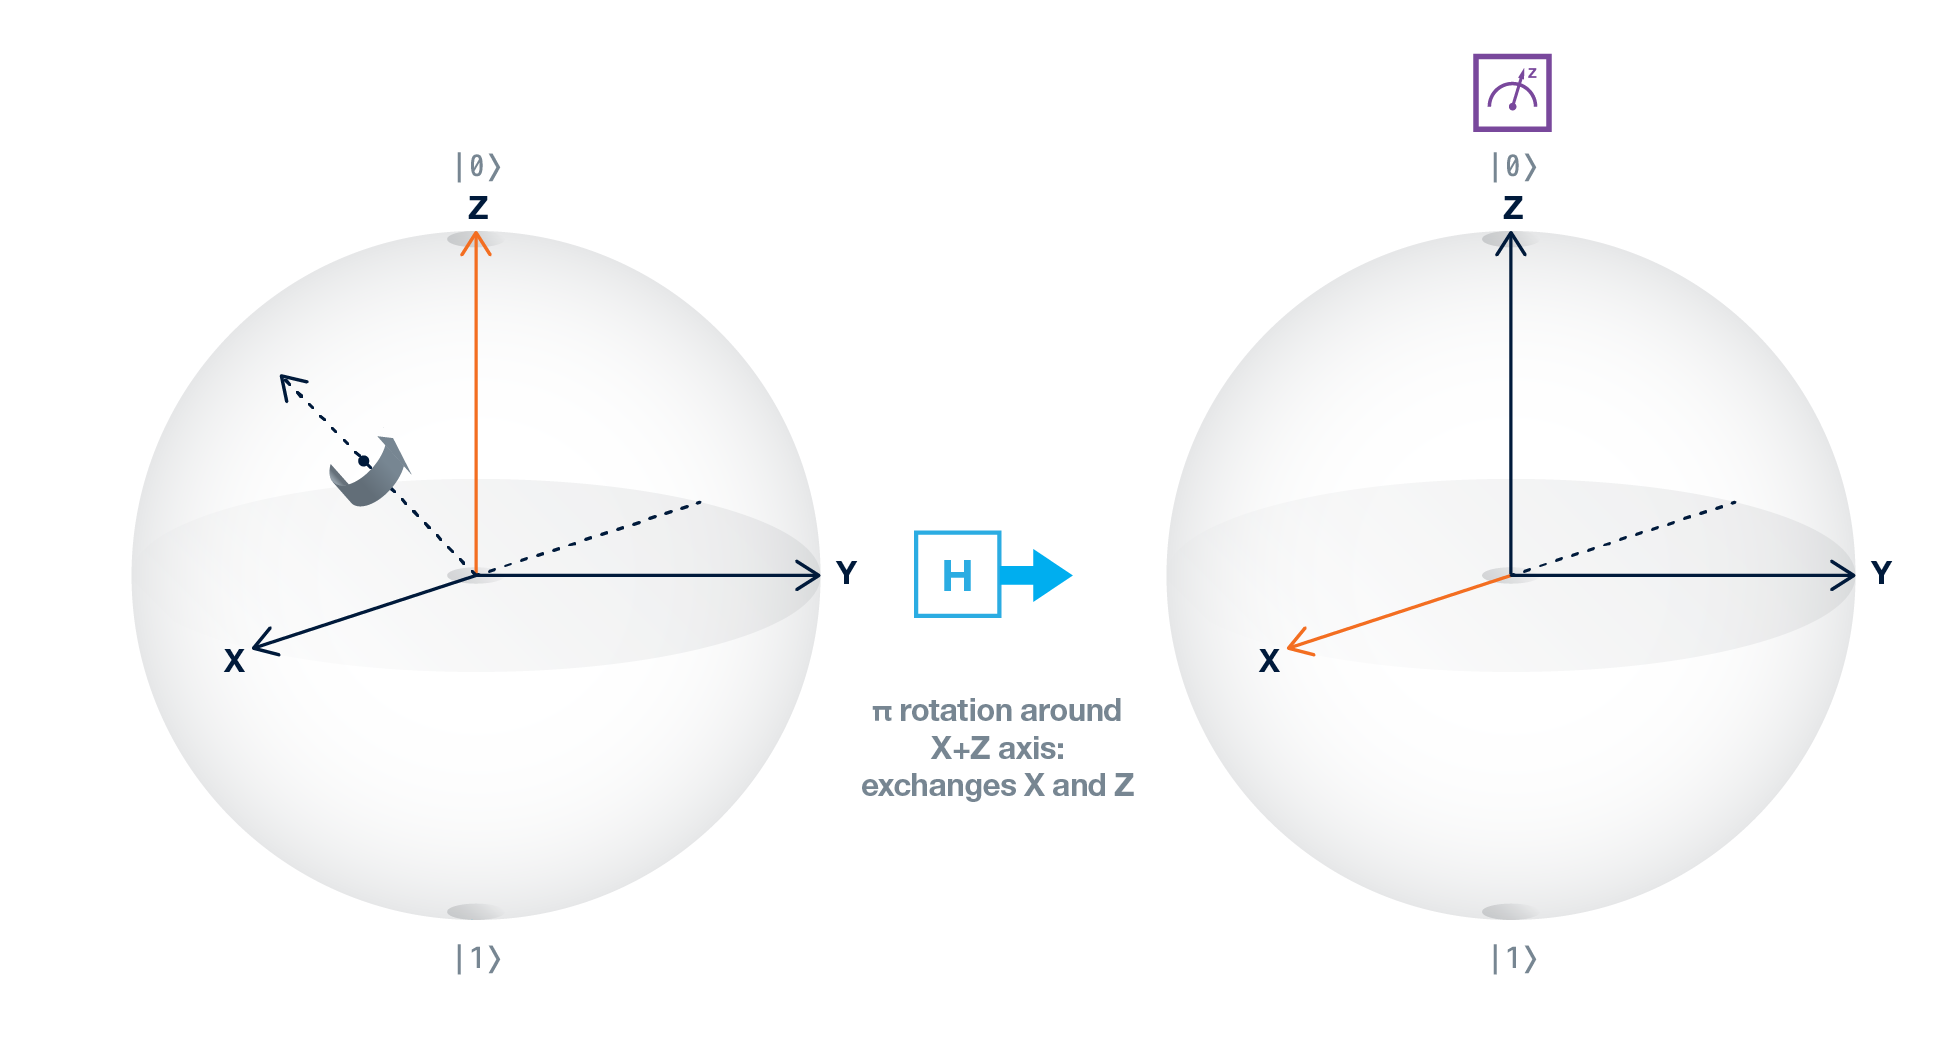
\includegraphics[width=\textwidth]{gate_h_bloch.png}
\end{frame}

\subsection{CNOT Gate}
\begin{frame}
    \frametitle{Controlled Not Gate}
    \centering
    \textbf{CNOT flips the \textit{target} bit if the \textit{control} bit is 1}
    \begin{equation*}
        \Qcircuit {
            \lstick{\ket{0}}  & \ctrl{1} & \rstick{\ket{0}} \qw \\ 
            \lstick{a\ket{0} + b\ket{1}} &  \targ & \rstick{a\ket{0} + b\ket{1}} \qw \\
    }
    \end{equation*}\\
    \vspace{3em}
    \begin{equation*}
        \Qcircuit {
            \lstick{\ket{1}} & \ctrl{1} & \rstick{\ket{1}} \qw\\ 
            \lstick{a\ket{0} + b\ket{1}} & \targ & \rstick{b\ket{0} + a\ket{1}} \qw\\
    }
    \end{equation*}
\end{frame}

\subsection{Quantum Circuits}
\begin{frame}
    \frametitle{Quantum Circuits}
    \textbf{Putting it together you build a circuit like:}
    \begin{equation*}
        \Qcircuit @C=0.5em @R=0.0em @!R {
            \lstick{q0_{2}: \ket{0}} & \gate{X} & \gate{H} & \ctrl{2} &\qw & \meter & \qw & \qw & \qw & \qw\\
        \lstick{q0_{1}: \ket{0}} & \gate{X} & \gate{H} & \qw & \qw & \qw & \meter & \qw & \qw\\
        \lstick{q0_{0}: \ket{0}} & \qw & \gate{H} & \targ &  \qw & \qw & \qw & \meter & \qw & \qw\\
	 	\lstick{c0_{2}: 0} & \cw & \cw & \cw & \cw & \cw \cwx[-3] & \cw & \cw & \cw & \cw\\
	 	\lstick{c0_{1}: 0} & \cw & \cw & \cw & \cw & \cw & \cw \cwx[-3] & \cw & \cw & \cw\\
	 	\lstick{c0_{0}: 0} & \cw & \cw & \cw & \cw & \cw & \cw & \cw \cwx[-3] & \cw & \cw\\
	 }
    \end{equation*}
    \begin{itemize}
        \item Each row represents a bit, either quantum or classical
        \item The operations are performed each qubit left to right
        \item Shows dependencies of operations
    \end{itemize}
\end{frame}

\section{Example Application}
\begin{frame}
    \frametitle{Bernstein-Vazirani Algorithm\footnotemark}
    \begin{columns}
        \column{.3\textwidth}
            \centering
            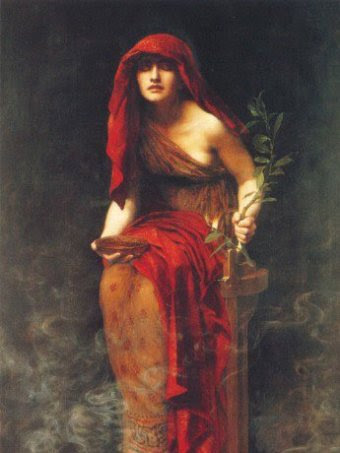
\includegraphics[width=\textwidth]{the_oracle.jpg} \\
            \large \textbf{The Oracle}
        \column{.7\textwidth}
        Input (query)\\
        $\Longleftarrow X_{n-1} \dotsb \ X_{1} X_{0} $\\
        \vspace{1.5em}
        Secret Bitstring\\
        $ \boxed{S_{n-1} \dotsb S_{1} S_{0}} $\\
        \vspace{1.5em} 
        Output (result)\\ 
		$\Longrightarrow X_{n-1}S_{n-1} \oplus \dotsb X_{1}S_{1} \oplus X_{0}S_{0} $\\
    \end{columns}
    \vspace{3em}
    \footnotetext[1]{E. Bernstein \& U. Vazirani, STOC, 93}
\end{frame}

\begin{frame}
    \frametitle{Optimal Classical Oracle}
	\begin{columns}
        \begin{column}{.3\textwidth}
            \centering
            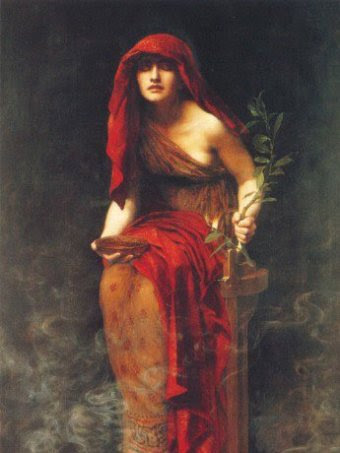
\includegraphics[width=\textwidth]{the_oracle.jpg}
        \end{column}
        \begin{column}{.7\textwidth}
            \centering
            Loop over each bit!
            \begin{flushleft}
            \[\left \{
                \begin{array}{lr}
                    X = 1\>0 \dotsb 0\>0 & \color{ibm} (2^{n-1})\\
                    X = 0\>1 \dotsb 0\>0 & \color{ibm} (2^{n-2})\\
                   \vdots  \\
                    X = 0\>0 \dotsb 1\>0 & \color{ibm} (2)\\
                    X = 0\>0 \dotsb 0\>1  & \color{ibm} (1)
                 \end{array}
               \right.
           \]
            \end{flushleft}
            \begin{center}
            \large \textbf{The ideal classical oracle is $\mathcal{O}(n)$}
            \end{center}
        \end{column}
    \end{columns}
\end{frame}

\begin{frame}
    \frametitle{Quantum Oracle}
    \begin{columns}
        \begin{column}{.3\textwidth}
            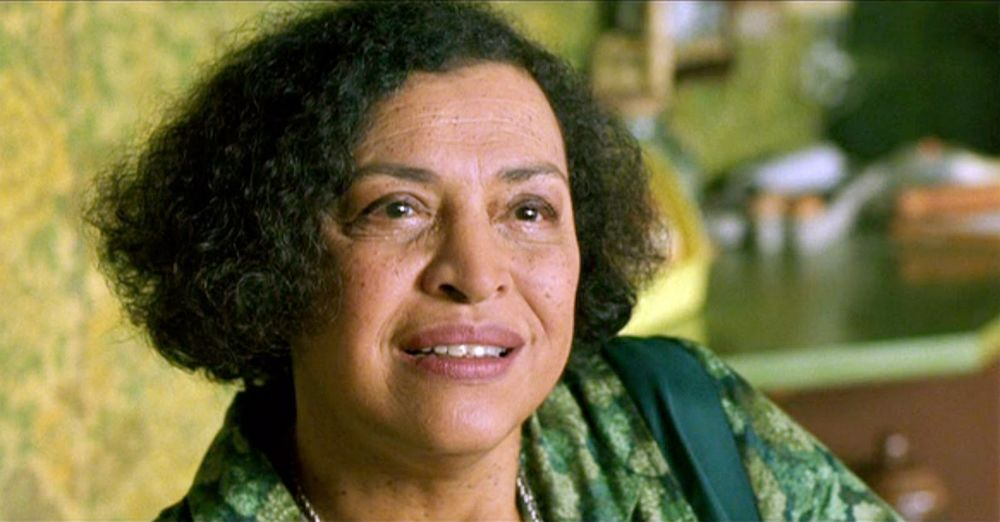
\includegraphics[width=1.2\textwidth]{quantum_oracle.jpg}
        \end{column}
        \begin{column}{.7\textwidth}
            \begin{equation*}
                \Qcircuit {
                    \lstick{\ket{x_{0}}} & \multigate{4}{Oracle} & \rstick{\ket{x_{0}}} \qw\\
                    \lstick{\ket{x_{1}}} & \ghost{Oracle} & \rstick{\ket{x_{1}}} \qw \\
                    \lstick{\ket{x_{2}}} & \ghost{Oracle} & \rstick{\ket{x_{2}}} \qw \\
                    \lstick{\ket{x_{3}}} & \ghost{Oracle} & \rstick{\ket{x_{3}}} \qw \\
                    \lstick{\ket{tmp}}   & \ghost{Oracle} & \rstick{\ket{x \cdot s} \oplus \ket{tmp}} \qw \\
                }
            \end{equation*}\\
            \begin{center}
                \large \textbf{A quantum oracle is $\mathcal{O}(1)$}
            \end{center}
        \end{column}
    \end{columns}
\end{frame}

\begin{frame}
    \frametitle{Quantum Oracle Implementation}
    \centering
    {\color{red}\textbf{$S = 1001$}}
    \begin{equation*}
        \Qcircuit {
            \lstick{\ket{x_{0}}} & \qw & \ctrl{4} & \qw  & \qw \\
            \lstick{\ket{x_{1}}} & \qw & \qw & \qw & \qw \\
            \lstick{\ket{x_{2}}} & \qw & \qw & \qw & \qw \\
            \lstick{\ket{x_{3}}} & \qw & \qw & \ctrl{1} & \qw \\
            \lstick{\ket{tmp}} & \qw & \targ & \targ & \qw
        }
    \end{equation*}
    {\color{red}1 \hspace{25pt} 0 \hspace{25pt} 0 \hspace{25pt} 1 \hspace{35pt} }\\
    $\ket{x_{3} \cdot s_{3} \oplus x_{2} \cdot s_{2} \oplus x_{1} \cdot s_{1} \oplus x_{0} \cdot s_{0} \oplus tmp}$
\end{frame}

\begin{frame}
    \frametitle{Full Circuit for a Quantum Oracle}
    \only<2>{
    \begin{equation*}
      \Qcircuit @C=0.5em @R=0.0em @!R {
           & & & & & \hspace{1em} \mbox{\textbf{The Oracle}} & & & & & & & & & & \\
           \lstick{q_{0}: \ket{0}} & \qw & \qw & \gate{H} & \qw & \ctrl{4} & \qw & \qw & \gate{H} & \qw & \qw & \qw & \qw & \meter & \qw & \qw\\
    	   \lstick{q_{1}: \ket{0}} & \qw & \qw & \gate{H} & \qw & \qw & \qw & \qw & \gate{H} & \qw & \qw & \qw & \meter & \qw & \qw & \qw\\
    	   \lstick{q_{2}: \ket{0}} & \qw & \qw & \gate{H} & \qw & \qw & \qw & \qw & \gate{H} & \qw & \qw & \meter & \qw & \qw & \qw & \qw\\
    	   \lstick{q_{3}: \ket{0}} & \qw & \qw & \gate{H} & \qw & \qw & \ctrl{1} & \qw & \gate{H} & \qw & \meter & \qw & \qw & \qw & \qw & \qw\\
    	   \lstick{tmp_{0}: \ket{0}} & \gate{X} & \qw & \gate{H} & \qw & \targ & \targ & \qw & \gate{H} & \qw & \qw & \qw & \qw & \qw & \qw & \qw\\
           \lstick{res_{0}: 0} & \cw & \cw & \cw & \cw & \cw & \cw & \cw & \cw & \cw & \cw & \cw & \cw & \cw \cwx[-5] & \cw & \cw & \rstick{1}\\
    	   \lstick{res_{1}: 0} & \cw & \cw & \cw & \cw & \cw & \cw & \cw & \cw & \cw & \cw & \cw & \cw \cwx[-5] & \cw & \cw & \cw & \rstick{0}\\
    	   \lstick{res_{2}: 0} & \cw & \cw & \cw & \cw & \cw & \cw & \cw & \cw & \cw & \cw & \cw \cwx[-5] & \cw & \cw & \cw & \cw & \rstick{0}\\
           \lstick{res_{3}: 0} & \cw & \cw & \cw & \cw & \cw & \cw & \cw & \cw & \cw & \cw \cwx[-5] & \cw & \cw & \cw & \cw & \cw & \rstick{1} \gategroup{2}{5}{6}{8}{.9em}{^\}}
    	 }
    \end{equation*}
    }
    \only<1>{
    \begin{equation*}
      \Qcircuit @C=0.5em @R=0.0em @!R {
           \lstick{q_{0}: \ket{0}} & \qw & \qw & \gate{H} & \qw & \multigate{4}{Oracle} & \qw & \gate{H} & \qw & \qw & \qw & \qw & \meter & \qw & \qw\\
           \lstick{q_{1}: \ket{0}} & \qw & \qw & \gate{H} & \qw & \ghost{Oracle} & \qw & \gate{H} & \qw & \qw & \qw & \meter & \qw & \qw & \qw\\
           \lstick{q_{2}: \ket{0}} & \qw & \qw & \gate{H} & \qw & \ghost{Oracle} & \qw & \gate{H} & \qw & \qw & \meter & \qw & \qw & \qw & \qw\\
           \lstick{q_{3}: \ket{0}} & \qw & \qw & \gate{H} & \qw & \ghost{Oracle} & \qw & \gate{H} & \qw & \meter & \qw & \qw & \qw & \qw & \qw\\
           \lstick{tmp_{0}: \ket{0}} & \gate{X} & \qw & \gate{H} & \qw & \ghost{Oracle} & \qw & \gate{H} & \qw & \qw & \qw & \qw & \qw & \qw & \qw\\
           \lstick{res_{0}: 0} & \cw & \cw & \cw & \cw & \cw & \cw & \cw & \cw & \cw & \cw & \cw & \cw \cwx[-5] & \cw & \cw & \rstick{1}\\
    	   \lstick{res_{1}: 0} & \cw & \cw & \cw & \cw & \cw & \cw & \cw & \cw & \cw & \cw & \cw \cwx[-5] & \cw & \cw & \cw & \rstick{0}\\
    	   \lstick{res_{2}: 0} & \cw & \cw & \cw & \cw & \cw & \cw & \cw & \cw & \cw & \cw \cwx[-5] & \cw & \cw & \cw & \cw & \rstick{0}\\
           \lstick{res_{3}: 0} & \cw & \cw & \cw & \cw & \cw & \cw & \cw & \cw & \cw \cwx[-5] & \cw & \cw & \cw & \cw & \cw & \rstick{1}
    	 }
    \end{equation*}
    }
    \only<2>{
    \centering
    \textbf{Where there is a CNOT phase kickback will set the control qubit to state \ket{1}}
    }
\end{frame}

\begin{frame}
    \frametitle{Live Demo}
\end{frame}


\section{Conclusion}
\subsection{Other Open Source Tools}
\begin{frame}
    \frametitle{Open Source in Quantum Computing}
    \begin{itemize}
        \item Many of the tools for developing quantum programs are open source
        \item Open source is used to help fosters collaboration
        \item Learning from the history of development of classical computers
        \item Many open source quantum computing projects already exist:
            \href{https://github.com/topics/quantum-computing}{https://github.com/topics/quantum-computing}
    \end{itemize}
\end{frame}

\begin{frame}
    \frametitle{Conclusions}
    \begin{itemize}
        \item Quantum Computing is about solving problems that we can't with
            classical computers
        \item It's still very early for quantum computers
        \item Not just in labs anymore, quantum computing is accessible by
            everyone now
        \item Open source software is playing a key role in the development of quantum computers
    \end{itemize}
\end{frame}

\section{Questions?}
\begin{frame}
\frametitle{Where to get more information}
    \begin{itemize}
        \item These Slides: \href{https://github.com/mtreinish/open-source-quantum-computing}{https://github.com/mtreinish/open-source-quantum-computing}
        \item Qiskit: \href{https://qiskit.org/}{https://qiskit.org/}
        \item Qiskit Terra on Github: \href{https://github.com/Qiskit/qiskit-terra}{https://github.com/Qiskit/qiskit-terra}
        \item IBM Q Experience: \href{https://quantumexperience.ng.bluemix.net/qx}{https://quantumexperience.ng.bluemix.net/qx}
        \item Tutorials on Quantum Computing and Qiskit: \href{https://github.com/Qiskit/qiskit-tutorials}{https://github.com/Qiskit/qiskit-tutorials}
    \end{itemize}
\end{frame}

\section{Backup Slides}
\begin{frame}[noframenumbering]
    \frametitle{BACKUP SLIDES}
\end{frame}
\section{Qubit Phase}
\begin{frame}[noframenumbering]
    \frametitle{Qubit Phase}
    \begin{columns}
    \column{.4\textwidth}
        \begin{itemize}
            \item While qubits are read along the basis vectors you can
                still use the other dimensions
            \item The phase can be leveraged to encode more information in the qubit
        \end{itemize}
        \column{.6\textwidth}
            \centering
            \textbf{Phase is $\phi$:}
            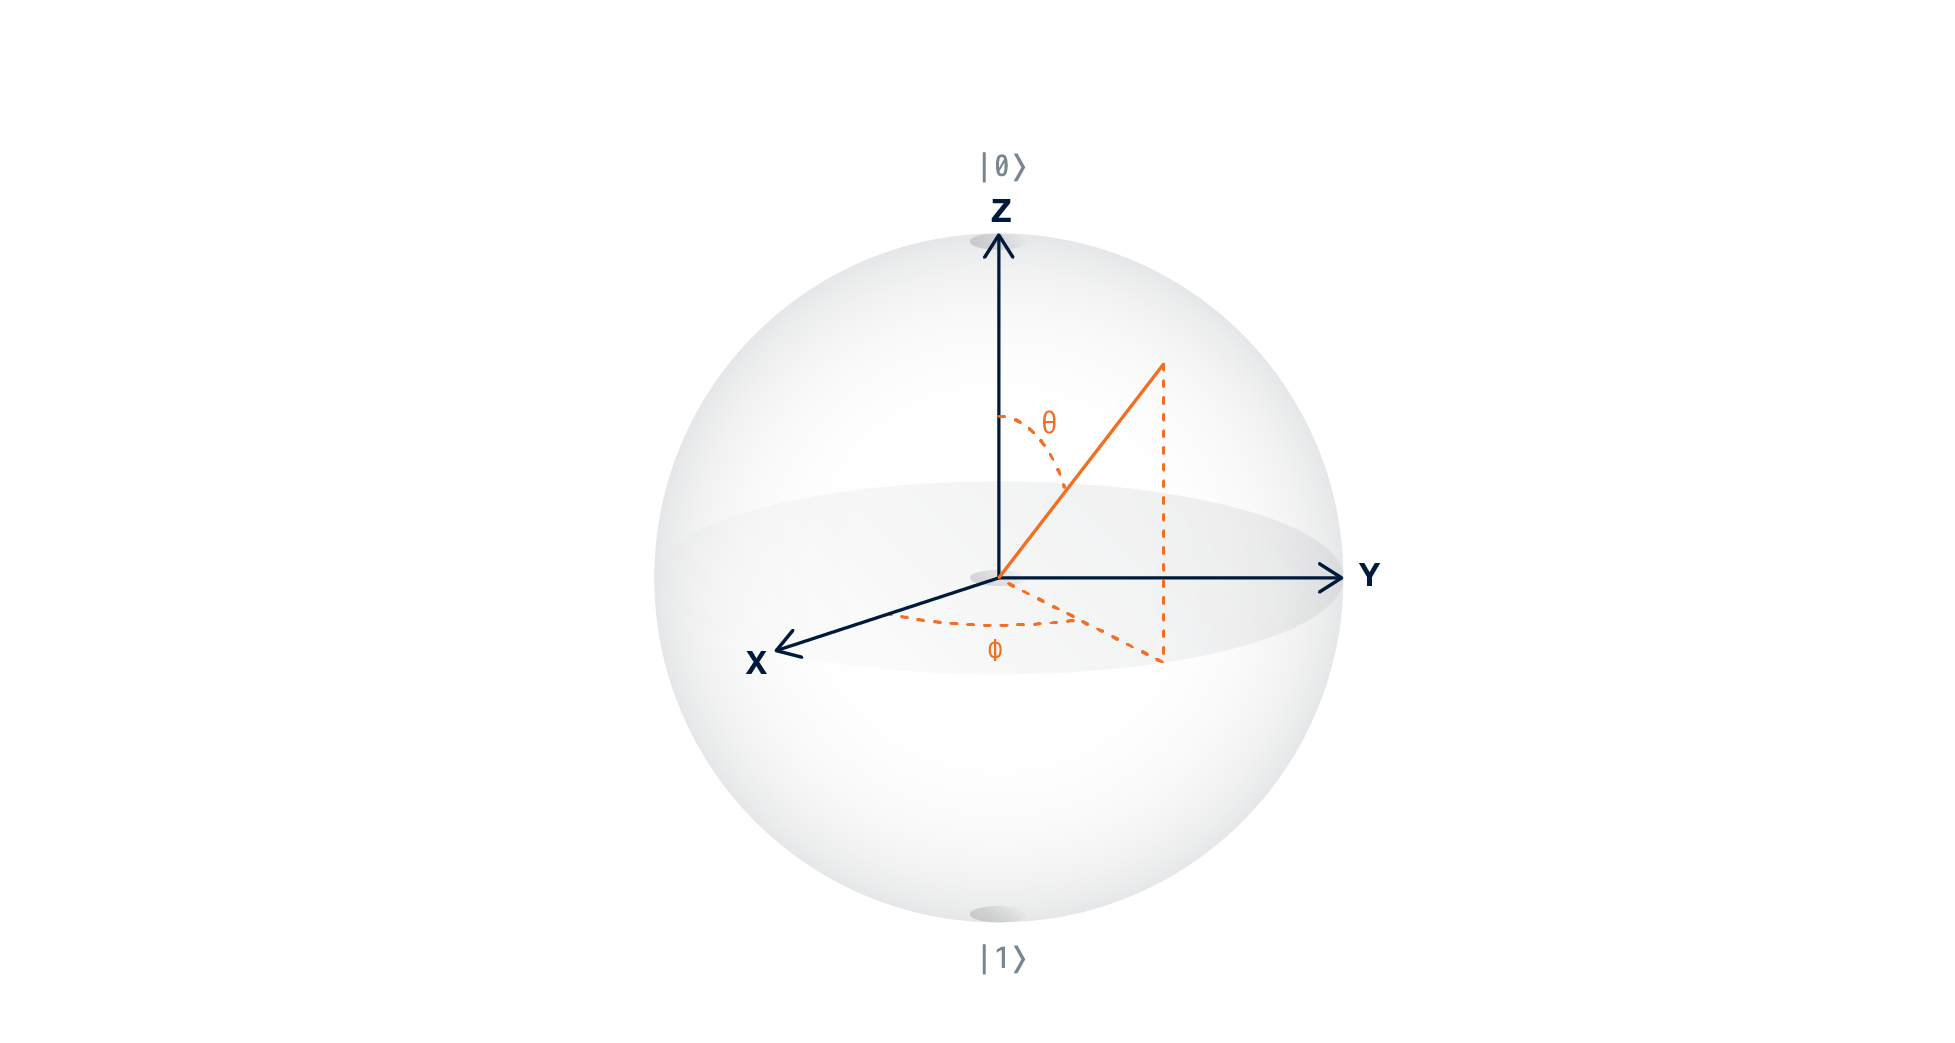
\includegraphics[height=.85\textwidth]{bloch_angles.png}
    \end{columns}
\end{frame}
\subsection{Hadamard and Phase}
\begin{frame}[noframenumbering]
    \frametitle{Hadamard and Phase}
    \textbf{Hadamard gates are self inverses:}
    \centering
    \begin{equation*}
        \Qcircuit {
            \lstick{\ket{0}} & \gate{H} & \qw & \mbox{\ket{0} + \ket{1}} & \hspace{5em} & \gate{H} & \rstick{\ket{0}} \qw
        }
    \end{equation*} \\
    \begin{equation*}
        \Qcircuit {
            \lstick{\ket{1}} & \gate{H} & \qw & \mbox{\ket{0} {\color{red} \textbf{-}} \ket{1}} & \hspace{5em} & \gate{H} & \rstick{\ket{1}} \qw \\
            & & & \mbox{\color{red} Phase} & & &
        }
    \end{equation*}
\end{frame}

\section{Phase Kickback}
\begin{frame}[noframenumbering]
    \frametitle{Phase Kickback}
    \centering
    \only<1->{$(\ket{0} + \ket{1})(\ket{0}  - \ket{1})$}\onslide<2->{$ = \ket{00} - \ket{01} + \ket{10} - \ket{11}$}\\
    \only<2>{Expand it}
    \only<1-2>{
    \begin{equation*}
        \Qcircuit {
            \lstick{\ket{0}} & \gate{H} \barrier[-1.65em]{1} & \qw \\
            \lstick{\ket{1}} & \gate{H} & \qw\\
        }
    \end{equation*}
    }
    \only<3-4>{
    \begin{equation*}
        \Qcircuit {
            \lstick{\ket{0}} & \gate{H} \barrier[-1.65em]{1} & \ctrl{1} & \qw\\
            \lstick{\ket{1}} & \gate{H} & \targ & \qw \\
        }
        \end{equation*}
    }
    \only<5>{
    \begin{equation*}
        \Qcircuit {
            \lstick{\ket{0}} & \gate{H} \barrier[-1.65em]{1} & \ctrl{1} \barrier[-1.65em]{1} & \gate{H} & \rstick{\ket{1}} \qw\\
            \lstick{\ket{1}} & \gate{H} & \targ & \gate{H} & \rstick{\ket{1}} \qw\\
        }
    \end{equation*}
    }
    \only<3->{$\ket{00} - \ket{01} - \ket{10} + \ket{11}$}\only<4->{$ = (\ket{0} {\textbf{\color{red}-}} \ket{1})(\ket{0} - \ket{1})$}\\
    \only<4-5>{\color{red}Phase Kickback}

\end{frame}

\subsection{Machine Types}
\begin{frame}[noframenumbering]
    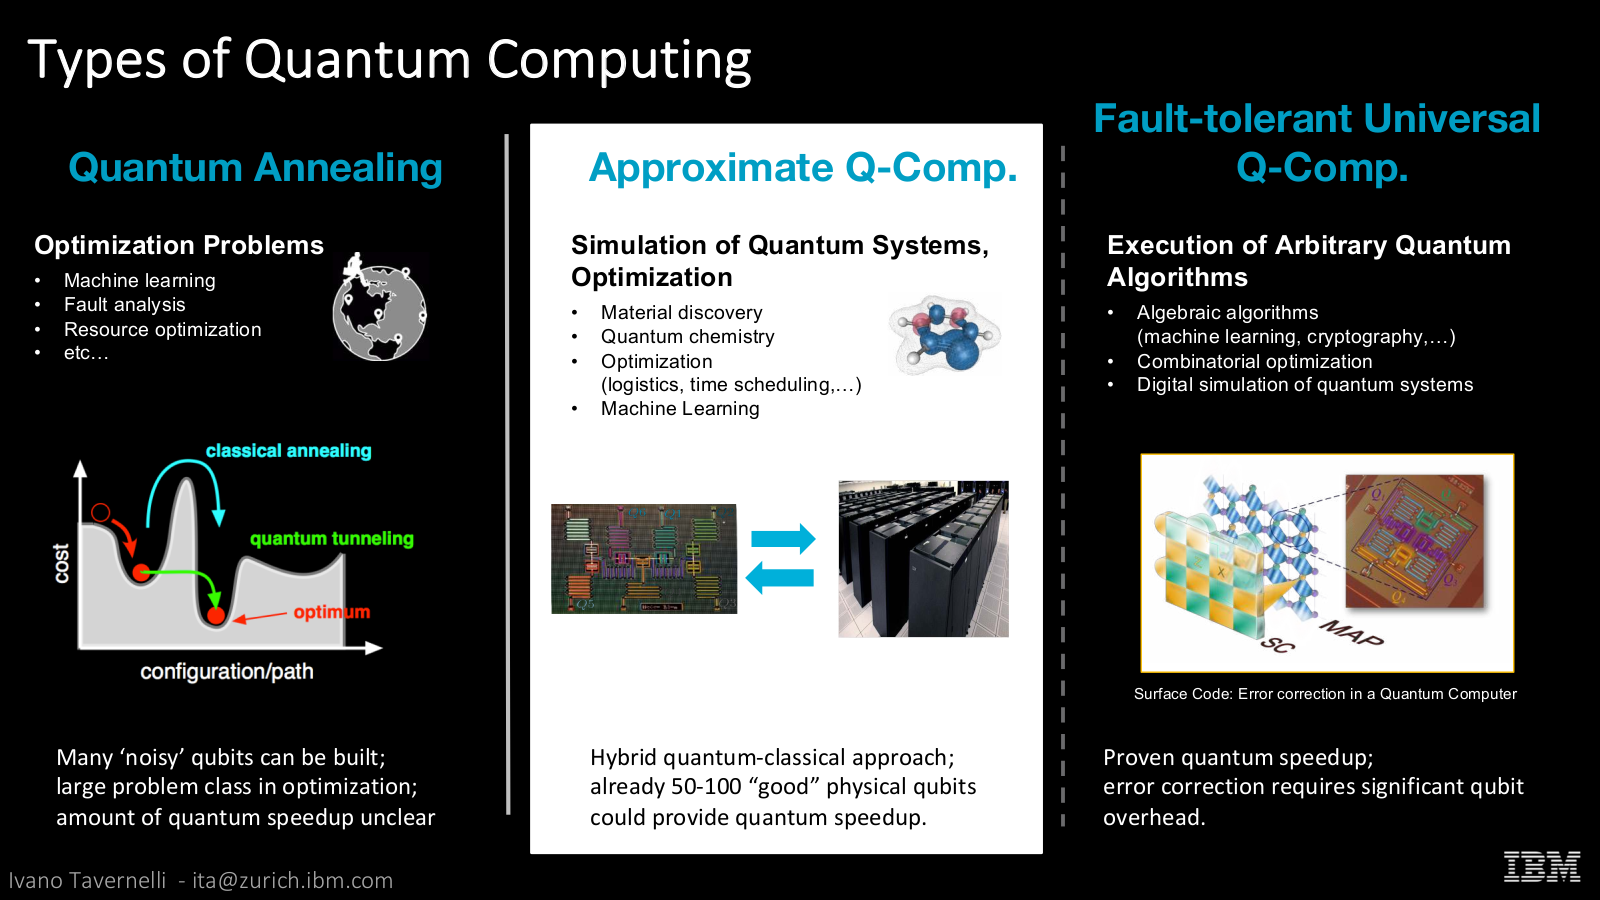
\includegraphics[width=\textwidth]{machine_types.png}
\end{frame}
\subsection{Entanglement}
\begin{frame}[noframenumbering]
    \frametitle{Entanglement}
    \begin{columns}
        \column{.45\textwidth}
            \begin{itemize}
                \item 2 qubits too far apart to influence each other can behave in a way that are \textbf{individually random} but are \textbf{strongly correlated}
                \item The state of an n-qubit system cannot (in general) be written as the state of its individual components.
                \item To simulate entanglement you need exponential resources
                \item CNOT gates are often used to setup entanglements
            \end{itemize}
        \column{.45\textwidth}
        \centering
            \textbf{One Qubit:}\\
            ${\color{ibm}a}\ket{0} + {\color{ibm}b}\ket{1}$\\
            \textbf{Two Qubits:}\\
            ${\color{ibm}a}\ket{00} + {\color{ibm}b}\ket{01} + {\color{ibm}c}\ket{11}$\\
            \textbf{Three Qubits:}\\
            ${\color{ibm}a}\ket{000} + {\color{ibm}b}\ket{001} + {\color{ibm}c}\ket{010} + {\color{ibm}d}\ket{011} + {\color{ibm}e}\ket{100} + {\color{ibm}f}\ket{101} + {\color{ibm}g}\ket{110} + {\color{ibm}h}\ket{111}$\\
    \end{columns}
\end{frame}


\end{document}
